\documentclass[11pt,a4paper]{article}

\usepackage[T1]{fontenc}
\usepackage{mathptmx}
\usepackage[scaled=0.9]{helvet}
\usepackage{courier}
\usepackage[margin=2.2cm]{geometry}
\usepackage{graphicx}
\usepackage{float}
\usepackage{booktabs}
\usepackage{amsmath,amssymb}
\usepackage{xcolor}
\usepackage[most]{tcolorbox}
\usepackage{listings}
\usepackage{caption}
\usepackage{enumitem}
\usepackage{needspace}
\usepackage{microtype}
\usepackage[colorlinks=true,linkcolor=blue!50!black,urlcolor=blue!50!black]{hyperref}

\graphicspath{{figures/}}
\captionsetup{font=small,labelfont=bf}
\setlength{\parskip}{0.55em}
\setlength{\parindent}{0pt}
\setlist{itemsep=0.15em,topsep=0.3em}

% ---------- boxes ----------
\newtcolorbox{answerbox}{breakable,colback=blue!4,colframe=blue!55!black,
  fonttitle=\bfseries,title=Answer,boxrule=0.6pt,arc=2pt,left=6pt,right=6pt,top=4pt,bottom=4pt}
\newtcolorbox{whybox}{breakable,colback=green!4,colframe=green!40!black,
  fonttitle=\bfseries,title=Why it looks like this,boxrule=0.6pt,arc=2pt,left=6pt,right=6pt,top=4pt,bottom=4pt}
\newtcolorbox{todobox}[1][TO COMPLETE before submitting]{breakable,colback=red!6,colframe=red!60!black,
  fonttitle=\bfseries,title=#1,boxrule=0.8pt,arc=2pt,left=6pt,right=6pt,top=4pt,bottom=4pt}

% ---------- code ----------
\lstset{language=Python,basicstyle=\ttfamily\footnotesize,keywordstyle=\color{blue!60!black},
  commentstyle=\color{gray},showstringspaces=false,frame=single,rulecolor=\color{black!25},
  breaklines=true,columns=fullflexible,xleftmargin=2pt,xrightmargin=2pt}

\newcommand{\sig}{\sigma}
\newcommand{\fc}{f_c}

\begin{document}

% =====================================================================
\begin{center}
  {\small Alexandria University \;|\; Faculty of Engineering \;|\; CCE: Computer Vision}\\[0.6em]
  {\LARGE\bfseries Assignment 1 --- Part 2}\\[0.3em]
  {\Large Frequencies, Pyramids and Blending}\\[0.8em]
\end{center}

\begin{todobox}[TO COMPLETE: team members (first page of the final PDF)]
Replace with the names and IDs of the three team members.

\medskip
\begin{tabular}{@{}ll@{}}
Member 1: & \texttt{[name]} \quad ID: \texttt{[id]}\\
Member 2: & \texttt{[name]} \quad ID: \texttt{[id]}\\
Member 3: & \texttt{[name]} \quad ID: \texttt{[id]}
\end{tabular}
\end{todobox}

\section*{Results at a glance}

\begin{center}
\small
\begin{tabular}{@{}lp{10.2cm}@{}}
\toprule
\textbf{Section} & \textbf{Main result}\\
\midrule
2.1 Hybrid images & $(\sig_{\text{low}},\sig_{\text{high}})$: man--cat $(10,5)$; pair~2 $(6,3)$; pair~3 $(6,3)$; pair~4 $(6,3)$ --- pair~4 (front face against profile) fails, as expected.\\
2.2 Aliasing & For a $4\times$ shrink of \texttt{rings.png} the smallest $\sigma$ with no visible false circles is $\sigma = 3$ (at $\sigma=2.5$ a faint residue is left at the borders).\\
2.3 Pyramids & Rebuild error $\max|I-\hat I| = 1.11\times10^{-16}$ (machine precision); the six-level Gaussian pyramid holds $1.3336\times$ the pixels of the image ($\to 4/3$).\\
2.4 Blending & Oraple: left-half mask, 6 levels. Face on a pumpkin: traced-outline mask (14.9\% of the image), 5 levels. Eye on the moon: traced-outline mask (5.8\%), 5 levels.\\
\bottomrule
\end{tabular}
\end{center}

\paragraph{Conventions used throughout.}
All blurs run on our own separable convolution with reflect padding (\texttt{np.pad(..., mode="reflect")}), as the
handout requires from Part~2 onward. Images are float64 in $[0,1]$; results are clipped to $[0,1]$ only for display.
Signed images (high-pass, Laplacian levels) are shown with zero as mid-gray. Our own images were resized so that the longer side is at most $1000$ pixels. Every section below has the same shape:
what we did, what came out, the \emph{answer} to the handout's question, and a short reflection on \emph{why} the
result looks the way it does.

% =====================================================================
\section{Hybrid images (2.1)}

\subsection{Method}
A hybrid keeps the low frequencies of an image $A$ and the high frequencies of an image $B$:
\begin{equation}
  H \;=\; \underbrace{G_{\sig_{\text{low}}} * A}_{\text{low-pass of }A}\;+\;\underbrace{\bigl(B - G_{\sig_{\text{high}}} * B\bigr)}_{\text{high-pass of }B},
\end{equation}
where $G_\sigma$ is a Gaussian of standard deviation $\sigma$ pixels. $B$ is first warped onto $A$ with
\texttt{align\_images.py} using two matching points (the eyes for the faces). The computation is done on grayscale
images, as in the handout figure.

A Gaussian of standard deviation $\sigma$ has frequency response $e^{-2\pi^2\sigma^2 f^2}$. We call its \emph{cutoff}
the frequency where the response drops to $e^{-1/2}\approx0.61$:
\begin{equation}
  \fc \;=\; \frac{1}{2\pi\sigma}\quad\text{cycles per pixel.}
\end{equation}
Larger $\sigma_{\text{low}}$ means a blurrier low image (lower cutoff); larger $\sigma_{\text{high}}$ means the high-pass
keeps \emph{less} (its cutoff moves down).

\begin{lstlisting}
def make_hybrid(im_low, im_high, sigma_low, sigma_high, clip=True):
    low  = gaussian_blur(im_low, sigma_low)
    high = im_high - gaussian_blur(im_high, sigma_high)
    hybrid = low + high
    return {..., "hybrid": np.clip(hybrid, 0, 1) if clip else hybrid}
\end{lstlisting}

\subsection{The three hybrids and their \texorpdfstring{$\sigma$}{sigma} values}

\begin{center}
\small
\begin{tabular}{@{}llcccccl@{}}
\toprule
Pair & Low-pass from / High-pass from & $\sig_{\text{low}}$ & $\sig_{\text{high}}$ & $\fc^{\text{low}}$ & $\fc^{\text{high}}$ & Outcome\\
\midrule
man--cat (starter) & man / cat & 10 & 5 & 0.016 & 0.032 & works\\
pair 2 (ours) & face A / face B & 6 & 3 & 0.027 & 0.053 & partial\\
pair 3 (ours) & smiling / serious (same person) & 6 & 3 & 0.027 & 0.053 & works well\\
pair 4 (ours) & front view / profile view & 6 & 3 & 0.027 & 0.053 & fails\\
\bottomrule
\end{tabular}
\end{center}

In all four pairs $\sigma_{\text{low}} = 2\sigma_{\text{high}}$, so the high-pass starts one octave above where the
low-pass ends. Frequencies in that gap are weak in \emph{both} layers, which is what keeps the two readings apart.

\subsection{Favorite pair: man and cat, the whole process}

\begin{figure}[H]
  \centering
  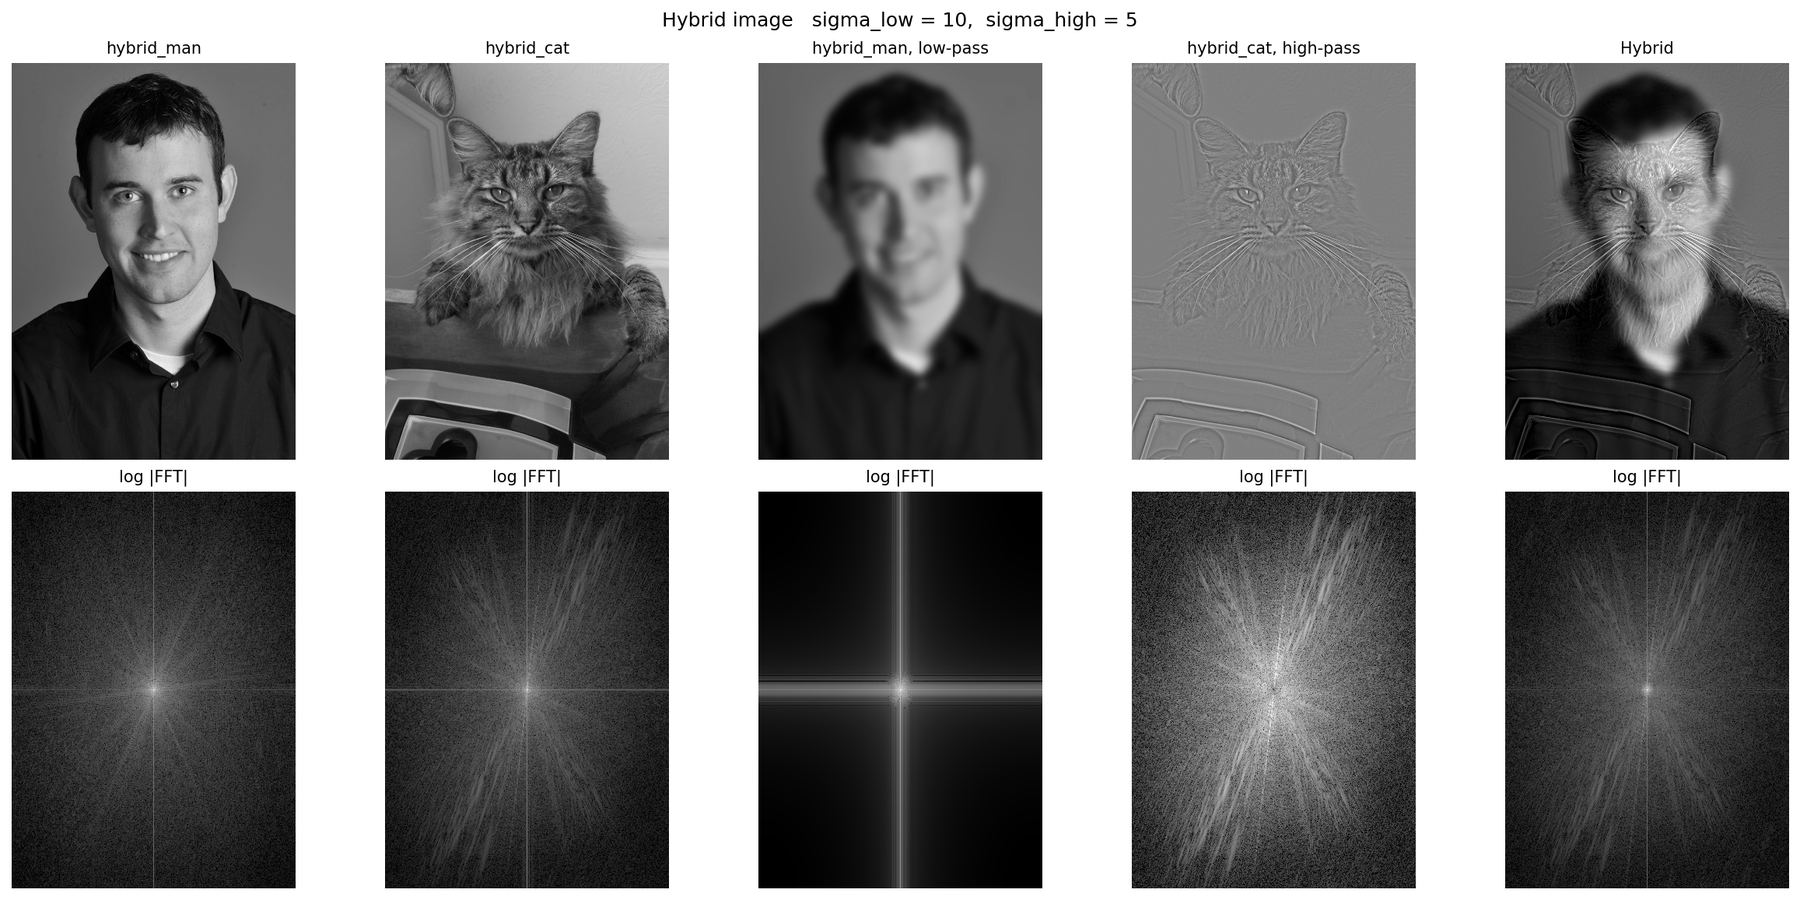
\includegraphics[width=\linewidth]{2_1_man_cat_report.png}
  \caption{Man (low-pass, $\sigma=10$) plus cat (high-pass, $\sigma=5$). Top: the two inputs, the two filtered images and the hybrid.
  Bottom: $\log|\mathrm{FFT}|$ of each, computed on the grayscale images with \texttt{np.log(np.abs(np.fft.fftshift(np.fft.fft2(gray))))}.}
\end{figure}

\begin{whybox}
\textbf{Reading the spectra.}
(i)~The man's low-pass spectrum is bright only close to the center and black elsewhere: everything above roughly
$0.016$ cycles/pixel was removed. (ii)~The cat's high-pass spectrum is the opposite: a dark spot at the center
(the low frequencies are gone) and energy spread over the whole plane. The streaks follow the orientation of the fur and the
whiskers. (iii)~The hybrid's spectrum looks like the man's near the center and like the cat's far from it, because the Fourier
transform is linear: $\mathcal{F}\{H\}=\mathcal{F}\{\text{low}\}+\mathcal{F}\{\text{high}\}$, and in each frequency region only one
of the two terms is large. (iv)~The bright horizontal and vertical cross in the blurred spectrum is not part of the picture:
the DFT treats the image as periodic, so the mismatch between opposite borders acts like a sharp edge and leaks energy along the two axes.

\textbf{Why the man is the low image and the cat the high one.} The man's face is smooth, so its identity lives in coarse
shapes (outline of the head, position of the eyes) that survive blurring. The cat's identity lives in fur and whiskers,
which are high-frequency texture. Swapping the roles would put a blurry cat under a face-sized pattern of skin pores.
\end{whybox}

\begin{figure}[H]
  \centering
  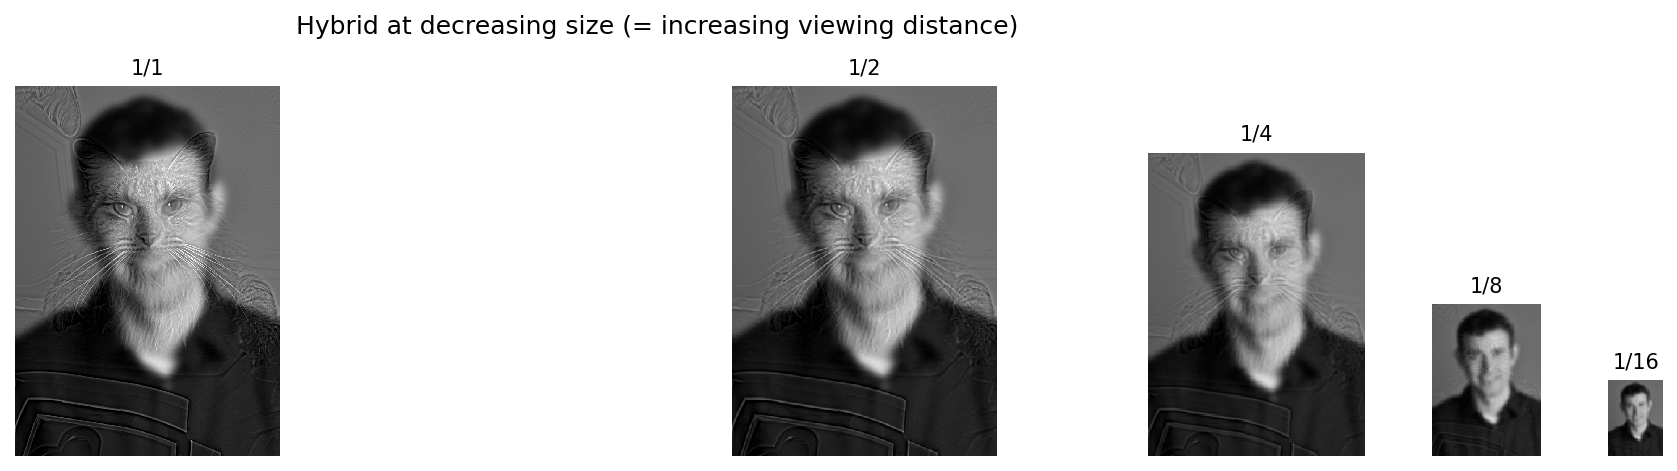
\includegraphics[width=\linewidth]{2_1_man_cat_distance.png}
  \caption{The hybrid shown at $1$, $1/2$, $1/4$, $1/8$ and $1/16$ of its size, each tile drawn at its true pixel size
  (a stand-in for increasing viewing distance). The cat dominates at $1$ and $1/2$; at $1/8$ and $1/16$ only the man remains.}
\end{figure}

\begin{whybox}
\textbf{Why identity changes with distance.} Shrinking an image by a factor $s$ multiplies all its spatial frequencies (in cycles per
pixel) by $s$, and the blur that precedes subsampling removes whatever no longer fits. The cat's fur, with features a few
pixels wide, is the first thing to disappear; the man's head, whose features are tens of pixels wide, is still resolved at $1/8$.
The eye does the same thing as we step back: it acts as a low-pass filter whose cutoff, measured in image coordinates, falls with distance.
\end{whybox}

\paragraph{Tuning $\sigma_{\text{low}}$ and $\sigma_{\text{high}}$.}
Figure~\ref{fig:sigmagrid} varies both. Reading across, a larger $\sigma_{\text{low}}$ blurs the man further, until at $16$ he is
a dark halo behind the cat. Reading down, a larger $\sigma_{\text{high}}$ lowers the cat's cutoff, so more mid-frequency cat
gets in, until at $9$ the cat is everywhere and the man is hard to find even from afar. The balance is best around
$(10,5)$: close up the cat is clear, from far away the man is clear, and neither layer hides the other.

\begin{figure}[H]
  \centering
  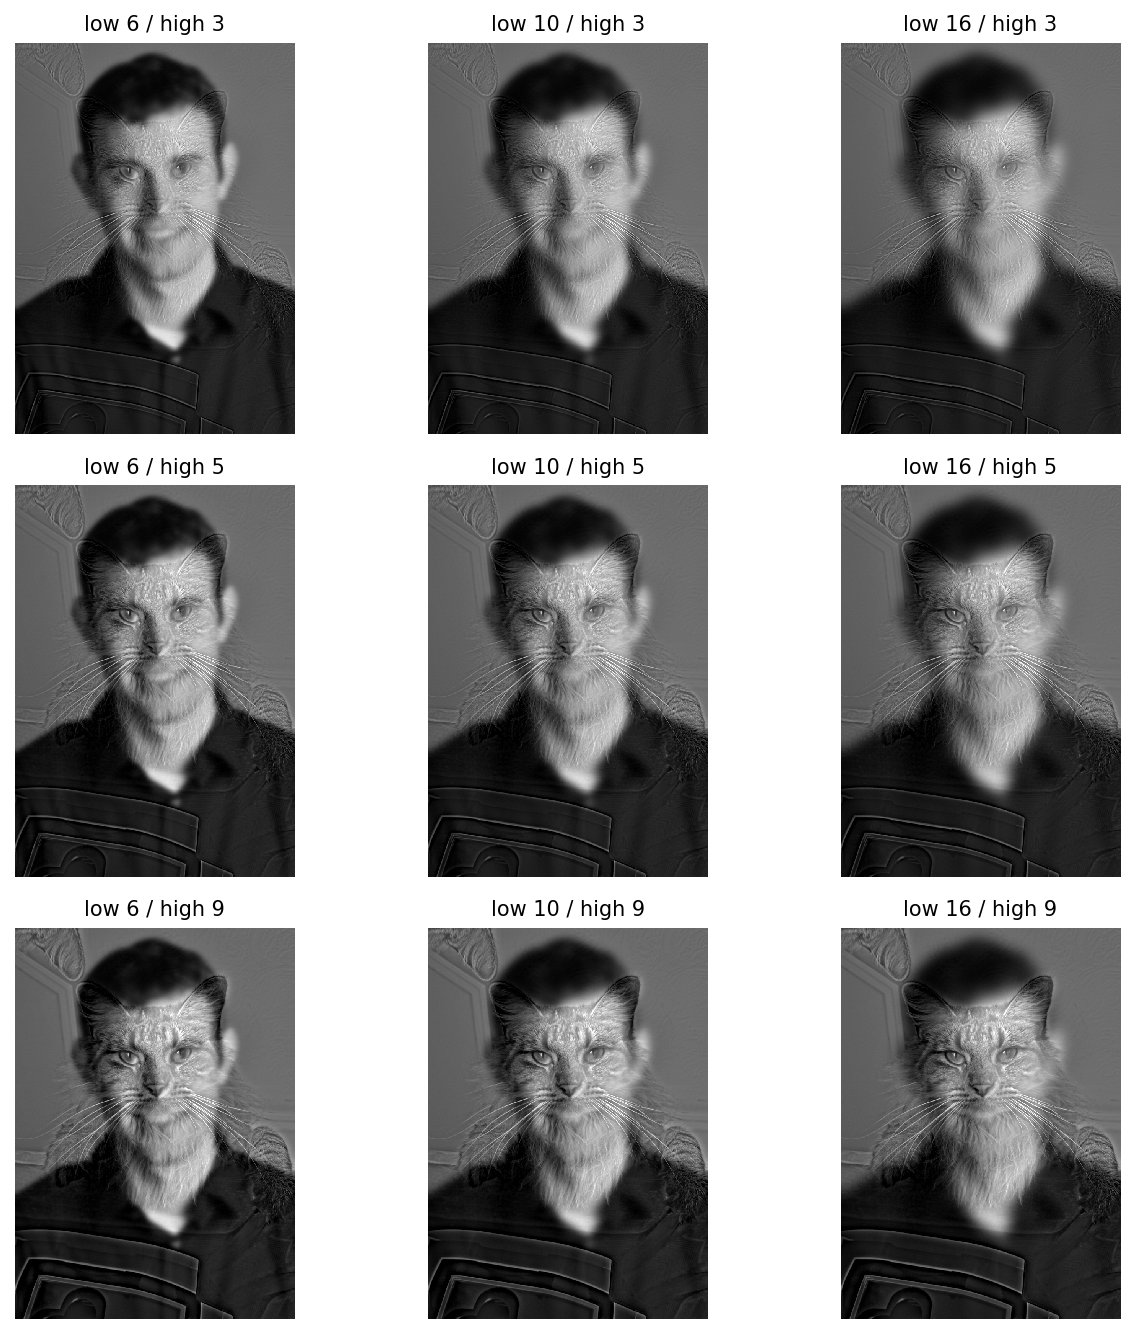
\includegraphics[width=0.6\linewidth]{2_1_man_cat_sigma_grid.png}
  \caption{Man--cat for $\sigma_{\text{low}}\in\{6,10,16\}$ (columns) and $\sigma_{\text{high}}\in\{3,5,9\}$ (rows).}
  \label{fig:sigmagrid}
\end{figure}

\subsection{Our own pairs}

\begin{figure}[H]
  \centering
  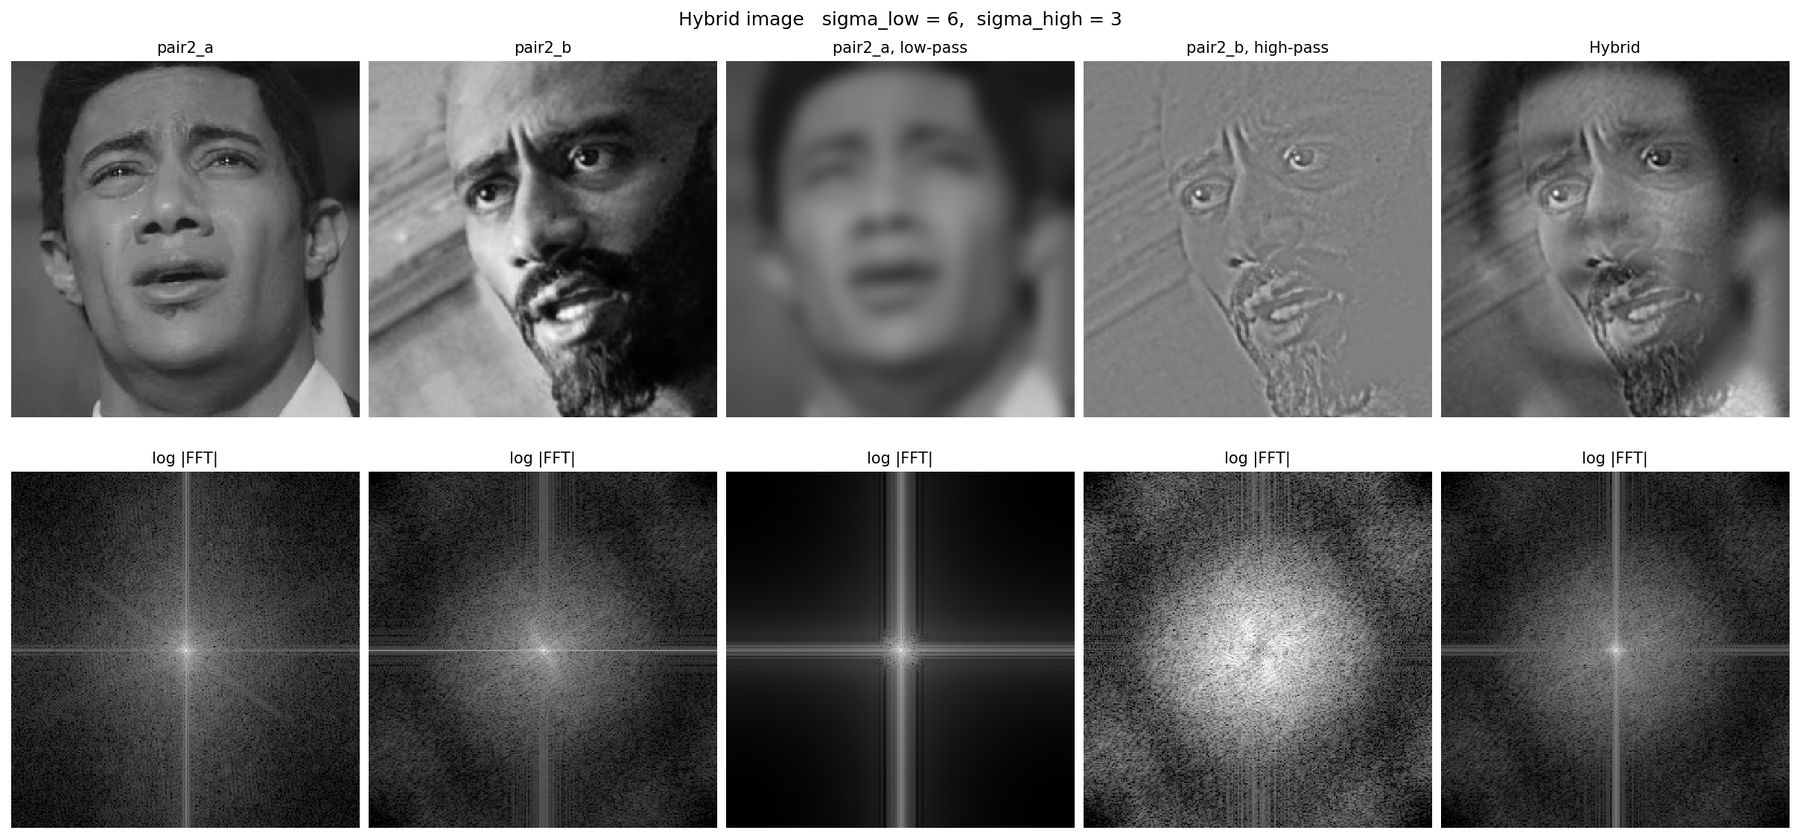
\includegraphics[width=\linewidth]{2_1_pair2_report.png}
  \caption{Pair 2, $\sigma_{\text{low}}=6$, $\sigma_{\text{high}}=3$.}
\end{figure}

\begin{figure}[H]
  \centering
  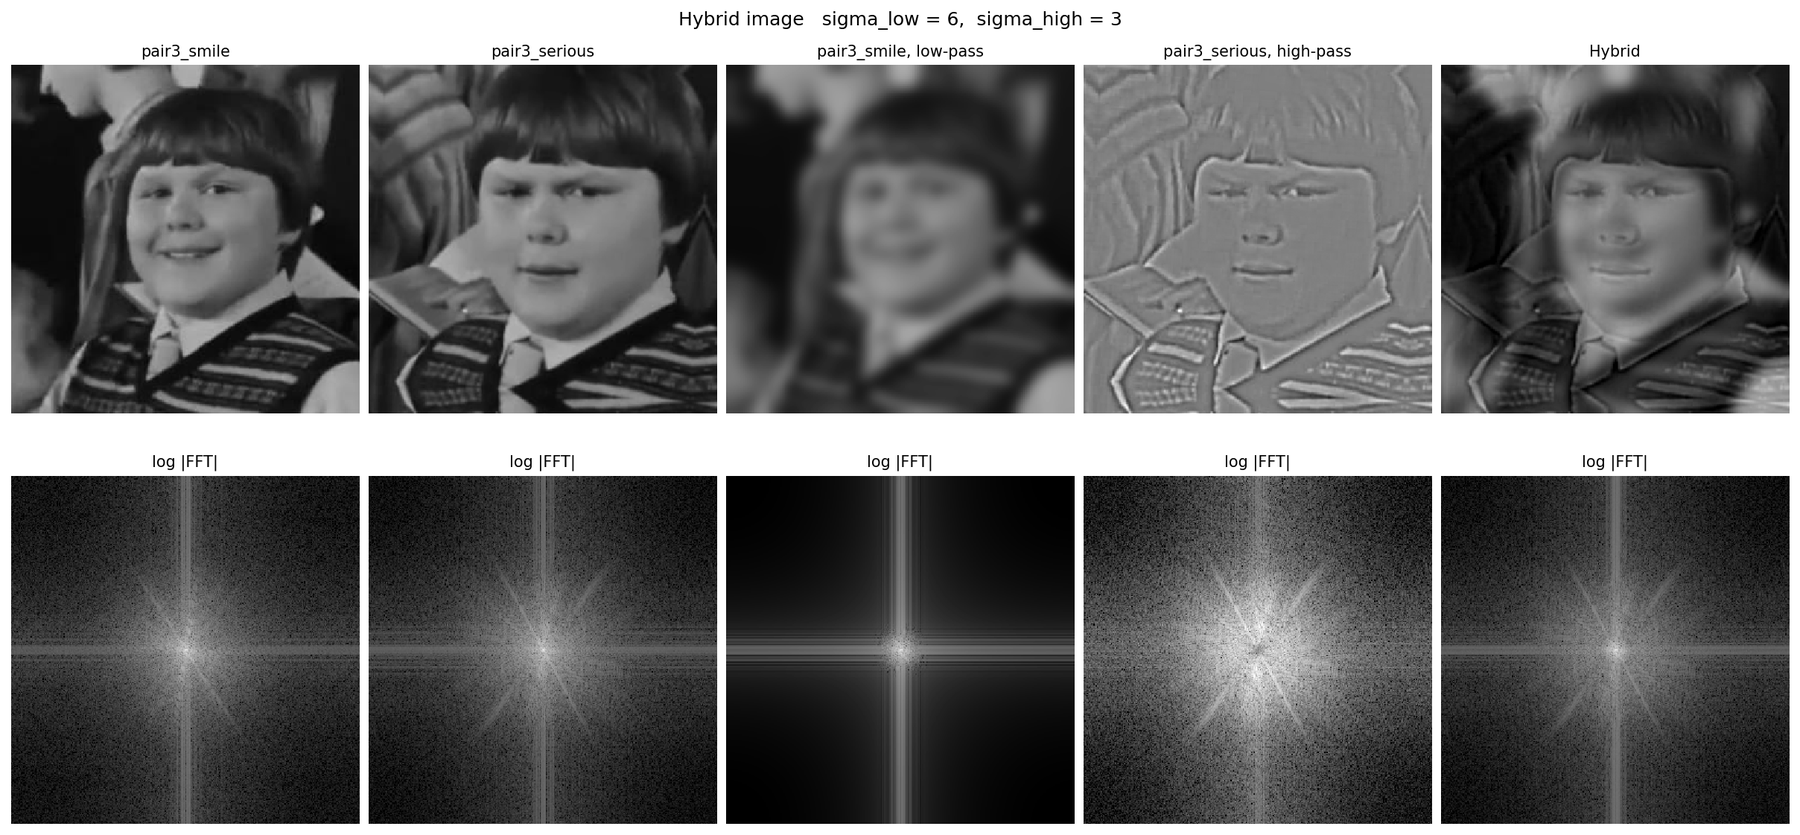
\includegraphics[width=\linewidth]{2_1_pair3_report.png}
  \caption{Pair 3 (same person, smiling and serious), $\sigma_{\text{low}}=6$, $\sigma_{\text{high}}=3$.}
\end{figure}

\begin{figure}[H]
  \centering
  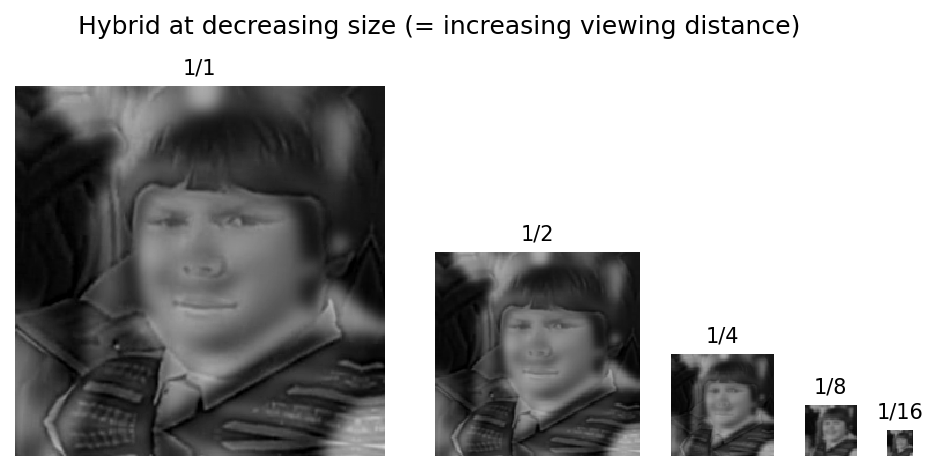
\includegraphics[width=0.8\linewidth]{2_1_pair3_distance.png}
  \caption{Pair 3 at decreasing size.}
\end{figure}

\begin{whybox}
\textbf{Pair 2 (partial).} The two eyes line up, because the eyes are the two alignment points. Away from the eyes
nothing is forced to match: the second head is tilted and its mouth and beard land on the first face's cheeks and chin, so the
hybrid reads as a face with an extra overlaid mouth rather than as one face. A two-point alignment is a similarity transform
(rotation, uniform scale, shift) and cannot correct a different head pose.

\textbf{Pair 3 (works best structurally).} The same person in the same pose: after the eyes are aligned, the brows,
nose, mouth and hairline of the two images already coincide, so the two layers fuse into one face. This is the ideal use of
the method: the high-pass layer re-draws the edges of the mouth and brows on top of the low-pass face, and the two layers
disagree only about the expression.
\end{whybox}

\subsection{The failing pair: front view against profile (pair 4)}

\begin{figure}[H]
  \centering
  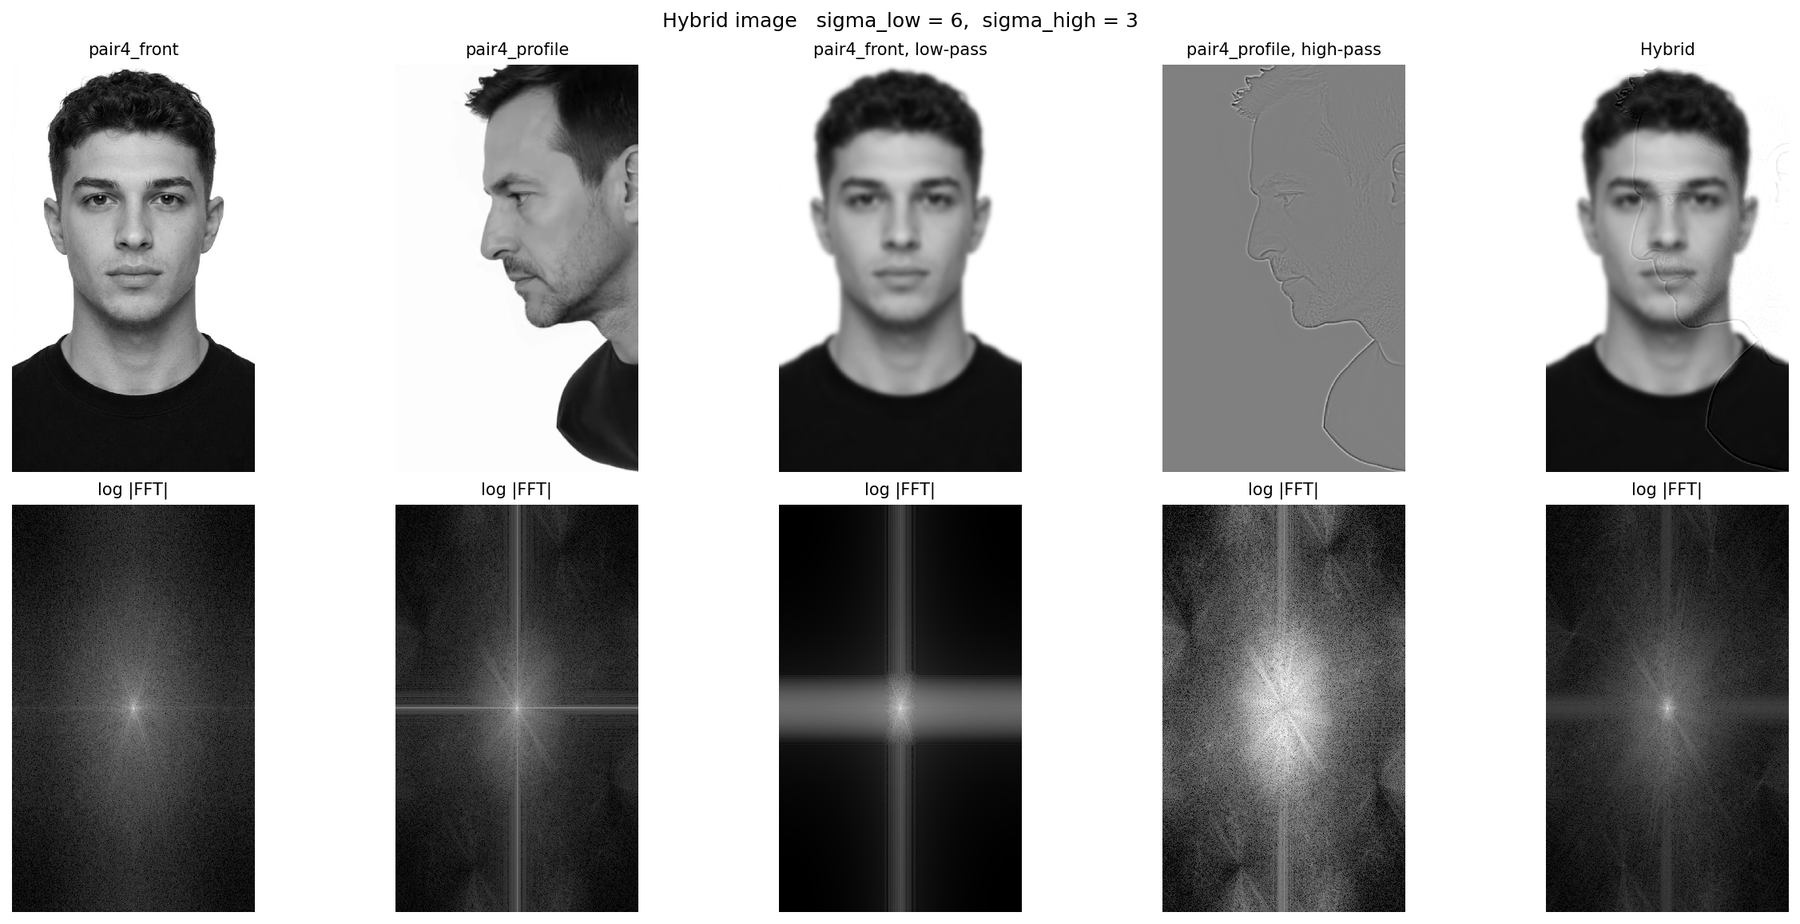
\includegraphics[width=\linewidth]{2_1_pair4_report.png}
  \caption{Pair 4: frontal face (low-pass) and profile (high-pass). The hybrid is essentially the frontal face with a few stray contour
  lines of the profile.}
\end{figure}

\begin{answerbox}
\textbf{Why does pair 4 fail?} Hybrid images need the two layers to be \emph{the same shape seen at two scales}. A
front view and a side view are different shapes: the nose, the lips and the ear are in different places, and the profile
face is cut by the image border. Two matching points can only rotate, scale and translate the second image; they cannot
turn a head. After the best possible alignment, the profile's edges do not sit on anything meaningful in the front face,
so they are read as scribbles, not as a second face.
\end{answerbox}

\begin{whybox}
The profile's high-pass is also nearly empty: the photo has a plain white background and smooth skin, so the only high-frequency content is the thin
silhouette line (see its spectrum, which is concentrated around the center). The hybrid therefore adds almost nothing to the frontal face except that outline.
It is a useful negative result: \emph{alignment of a few points is necessary for a hybrid, but it is the similarity of the two images' structure that makes
it work.}
\end{whybox}

% =====================================================================
\section{Aliasing (2.2)}

\subsection{Method}
Keeping every $k$-th pixel samples the image at $1/k$ samples per pixel, so the highest frequency it can still represent
(the new Nyquist limit) is
\begin{equation}
  f_N=\frac{1}{2k}\ \text{cycles per \emph{original} pixel}\qquad(f_N=0.125\ \text{for }k=4).
\end{equation}
Any component with $f>f_N$ is not lost: it \emph{folds} to a lower frequency $f'=|f-m/k|$ ($m$ the nearest integer) and is
indistinguishable from a genuine low-frequency component. Equivalently, the spectrum of the subsampled image is the original
spectrum copied at multiples of $1/k$; where the copies overlap, high-frequency energy lands in the low-frequency band.
Blurring first removes the energy above $f_N$ \emph{before} the copies are made.

\begin{figure}[H]
  \centering
  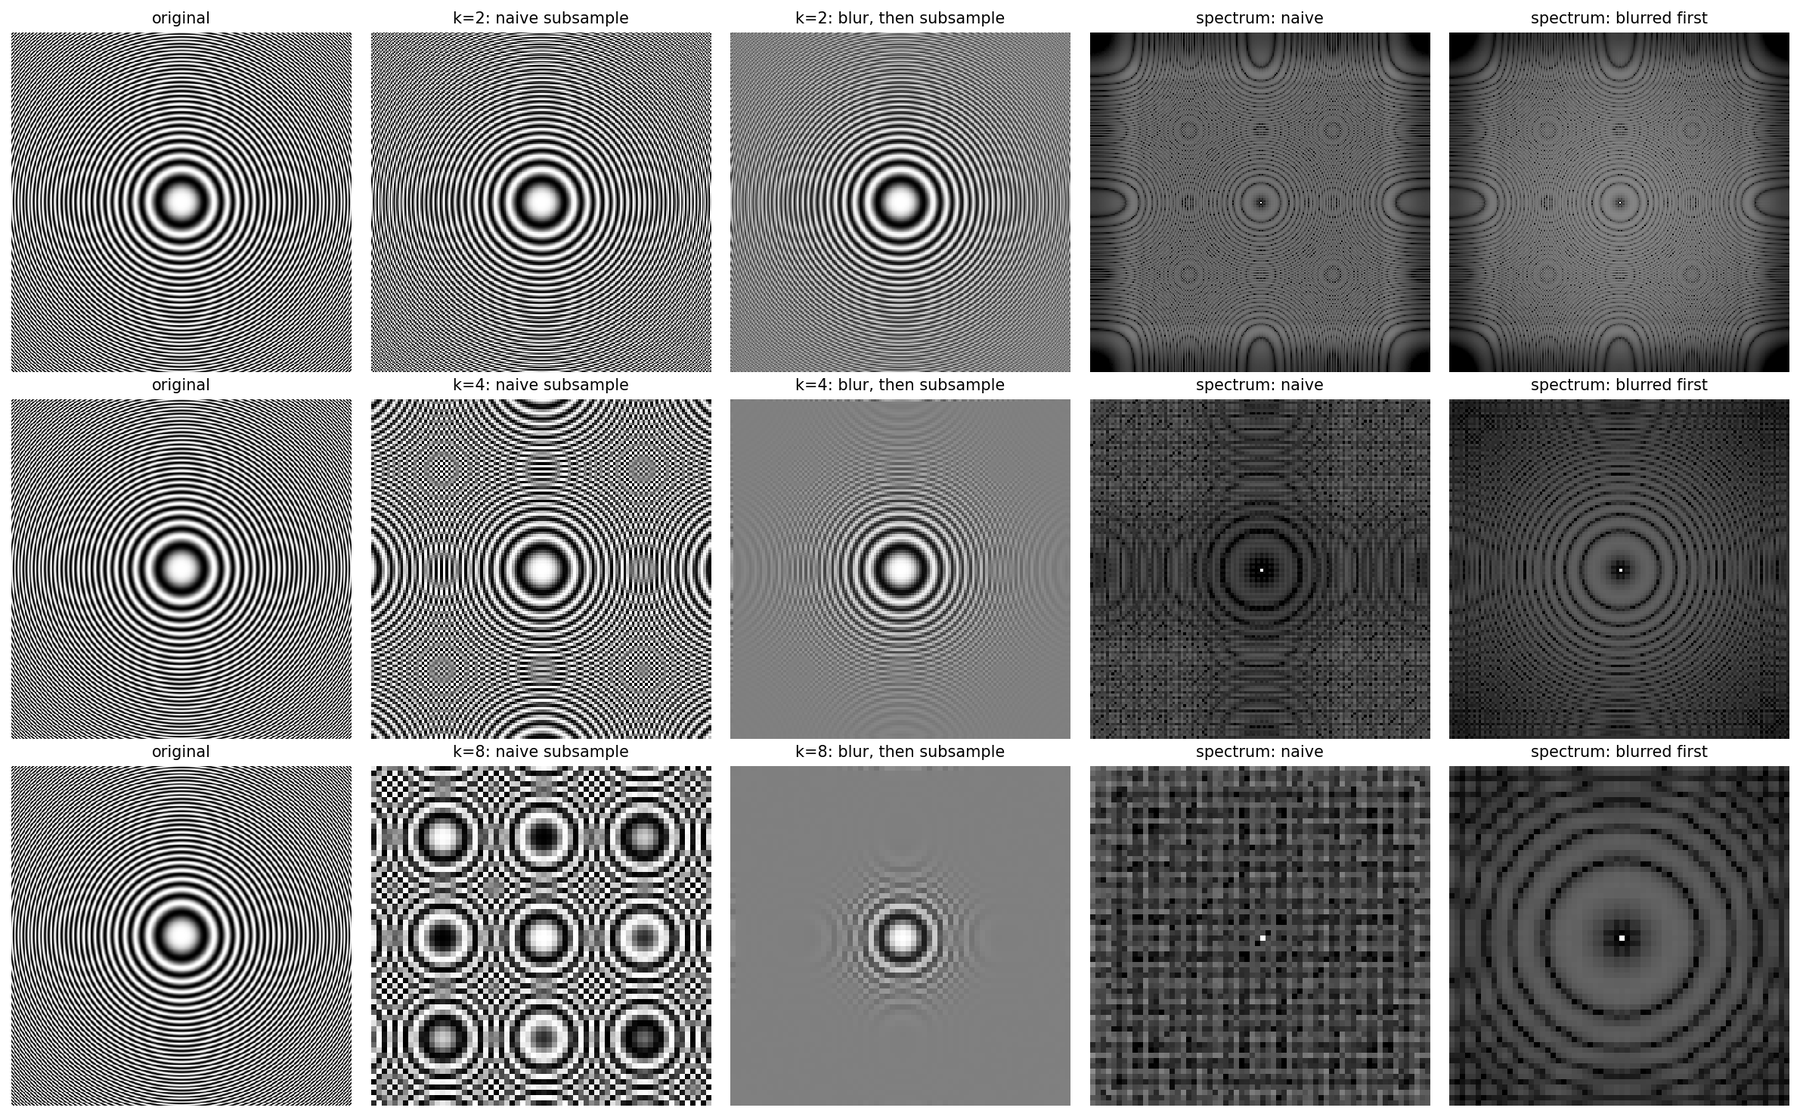
\includegraphics[width=\linewidth]{2_2_rings.png}
  \caption{\texttt{rings.png} shrunk by $k=2,4,8$: original, naive subsample, blur-then-subsample (with $\sigma=k/2$), and the spectrum
  of each. The shrunk images are blown back up to full size with nearest-neighbour pixels. Naive subsampling creates extra
  circle centers (moir\'e); blurring first does not.}
  \label{fig:rings}
\end{figure}

\subsection{The \texorpdfstring{$4\times$}{4x} shrink of \texttt{rings.png}}

\begin{figure}[H]
  \centering
  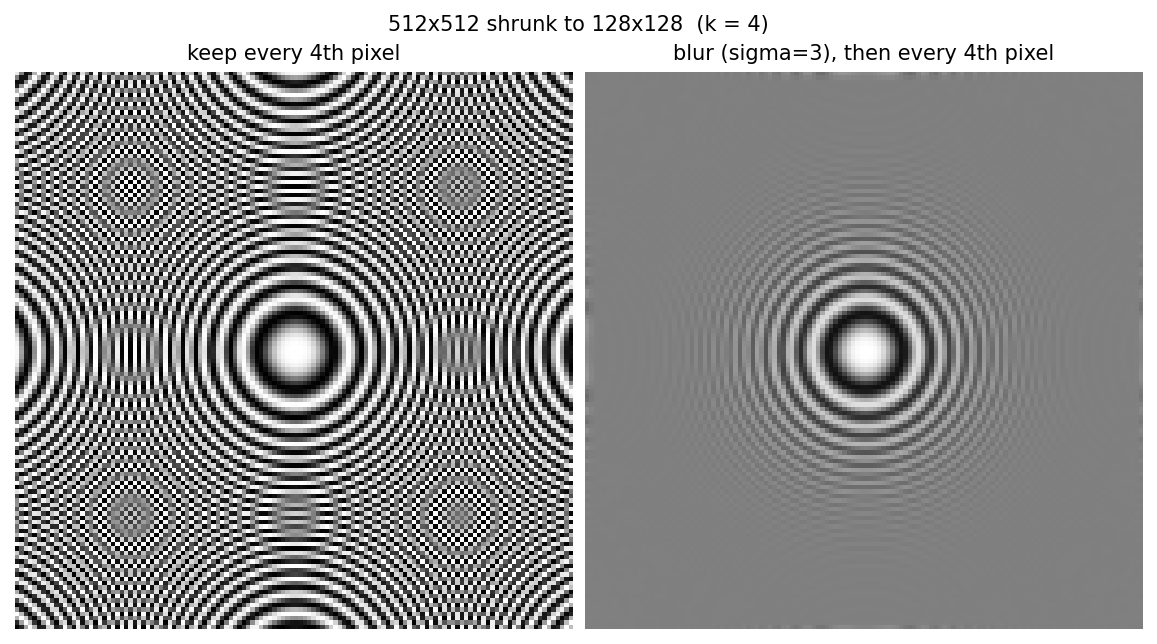
\includegraphics[width=0.85\linewidth]{2_2_rings_quarter.png}
  \caption{The two quarter-size results side by side ($512\times512\to128\times128$): left, keeping every 4th pixel; right,
  Gaussian blur with $\sigma=3$ and then every 4th pixel.}
\end{figure}

\begin{figure}[H]
  \centering
  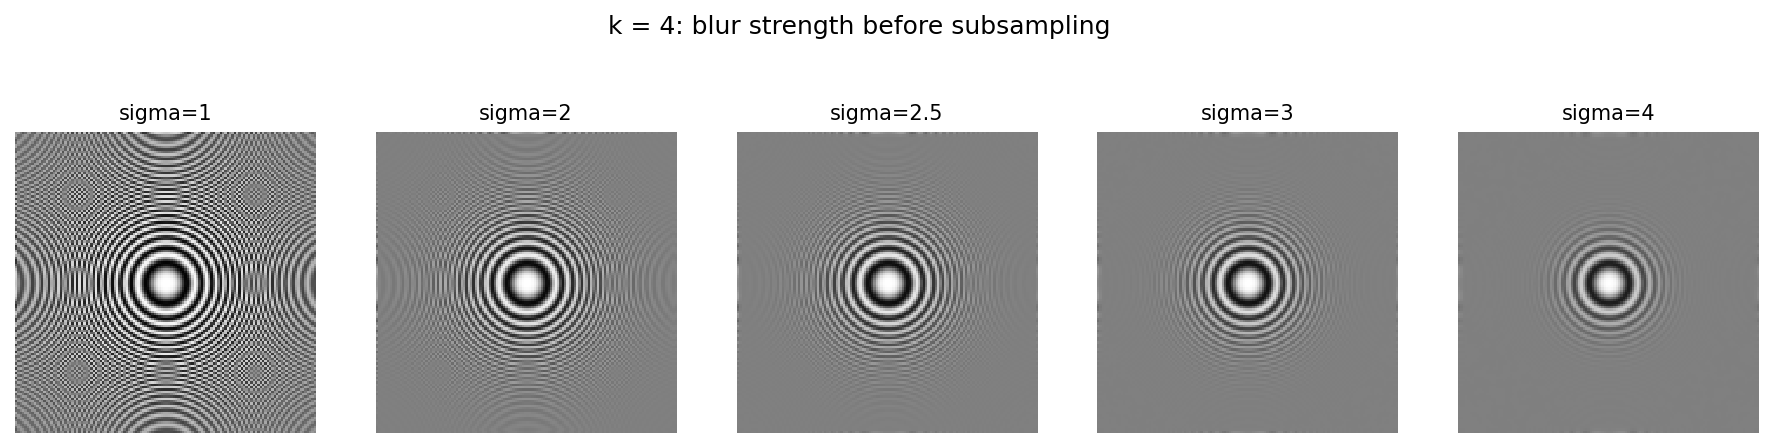
\includegraphics[width=\linewidth]{2_2_sigma_sweep.png}
  \caption{Blur strength before subsampling at $k=4$: $\sigma=1,2,2.5,3,4$ (shown at $4\times$ zoom).}
\end{figure}

To put a number next to the eye test: the outer rings of the original are far too fine to survive a $4\times$ shrink, so a correctly
anti-aliased result is flat gray there. Any contrast left in that region is false circles. Table~\ref{tab:sigma} gives the standard deviation of
the outer region (radius above $35\%$ of the image side) next to the Gaussian's response at the new Nyquist limit,
$H(f_N)=e^{-\pi^2\sigma^2/(2k^2)}$.

\begin{table}[H]
\centering
\small
\begin{tabular}{@{}lccccccccc@{}}
\toprule
 & naive & $\sigma{=}1$ & $1.5$ & $2$ & $2.5$ & $3$ & $3.5$ & $4$\\
\midrule
outer-ring std & 0.353 & 0.167 & 0.075 & 0.028 & 0.011 & 0.006 & 0.005 & 0.004\\
$H(f_N)$ & --- & 0.735 & 0.50 & 0.29 & 0.15 & 0.06 & 0.02 & 0.007\\
\bottomrule
\end{tabular}
\caption{Leftover false-circle contrast against blur strength, $k=4$.}
\label{tab:sigma}
\end{table}

\begin{answerbox}
\textbf{Smallest $\sigma$ with no false circles (for $k=4$): $\sigma=3$.}
At $\sigma=1$ the circles are still strong; at $\sigma=2$ faint arcs remain along the borders; at $\sigma=2.5$ a faint
residue is left at the top and bottom edges; at $\sigma=3$ none is visible, and the leftover contrast is $0.6\%$ of the range.

\textbf{What happened in each result.}
\emph{Keep every 4th pixel:} the rings with local frequency above $0.125$ cycles/pixel folded back into the representable
band. They reappear as coarse circles around eight extra centers (the points where the folded frequency passes through
zero), a pattern that is not in the original at all. The spectrum is the original spectrum copied and overlapped, so
energy fills the whole plane. \emph{Blur, then keep every 4th pixel:} the Gaussian removed the energy above $f_N$ first, so
there was nothing left to fold. What remains is the center of the pattern, which \emph{is} representable, and flat gray where the rings were too fine.
\end{answerbox}

\begin{whybox}
\textbf{Why $\sigma=3$ and not the textbook $k/2=2$.} A Gaussian is not a brick-wall filter: its response falls gradually.
With $\sigma=k/2=2$ the response at the new Nyquist limit is still $0.29$, so $29\%$ of the amplitude of the offending
frequencies survives and folds, which is the faint arcs we see. At $\sigma=3$ it is $0.06$. For this image a good rule is
therefore $\sigma\approx0.75\,k$ rather than $k/2$ (measured on this one image and this one $k$).

\textbf{Why not blur even more?} Over-blurring removes genuine detail. At $\sigma=4$ the false circles are gone, but the response at
\emph{half} the Nyquist limit is already $0.29$, so legitimate inner rings are weakened and the visible pattern shrinks.
The best $\sigma$ is the \emph{smallest} one that removes the aliasing, which is exactly the question the handout asks.
\end{whybox}

\begin{answerbox}
\textbf{What this means for a Gaussian pyramid.} Every reduction step must blur \emph{before} it subsamples, and the blur has to be
matched to the subsampling factor ($\sigma$ grows in proportion to $k$). Subsampling an unblurred level would put aliasing into the
pyramid, and every coarser level, every Laplacian level built from it and every blend that uses it would inherit it. In practice the
pyramid reduces by only a factor $2$ per step with a fixed small kernel, rather than by one large jump.
\end{answerbox}

\begin{whybox}
\textbf{An honest caveat about our own pyramid.} The $\frac1{16}[1\,4\,6\,4\,1]$ kernel of Section~\ref{sec:pyr} has variance $1$
(equivalent to $\sigma=1$) at $k=2$, where $f_N=0.25$. Its response there is $e^{-2\pi^2\cdot0.0625}=0.29$, the same $0.29$ as $\sigma=2$ at $k=4$.
So a single reduce step is not perfectly alias-free; it is the classic compromise (cheap, nearly separable, and small in extent), and what leaks through
is small and gets blurred again at the next level.
\end{whybox}

\subsection{A natural image confirms it}

\begin{figure}[H]
  \centering
  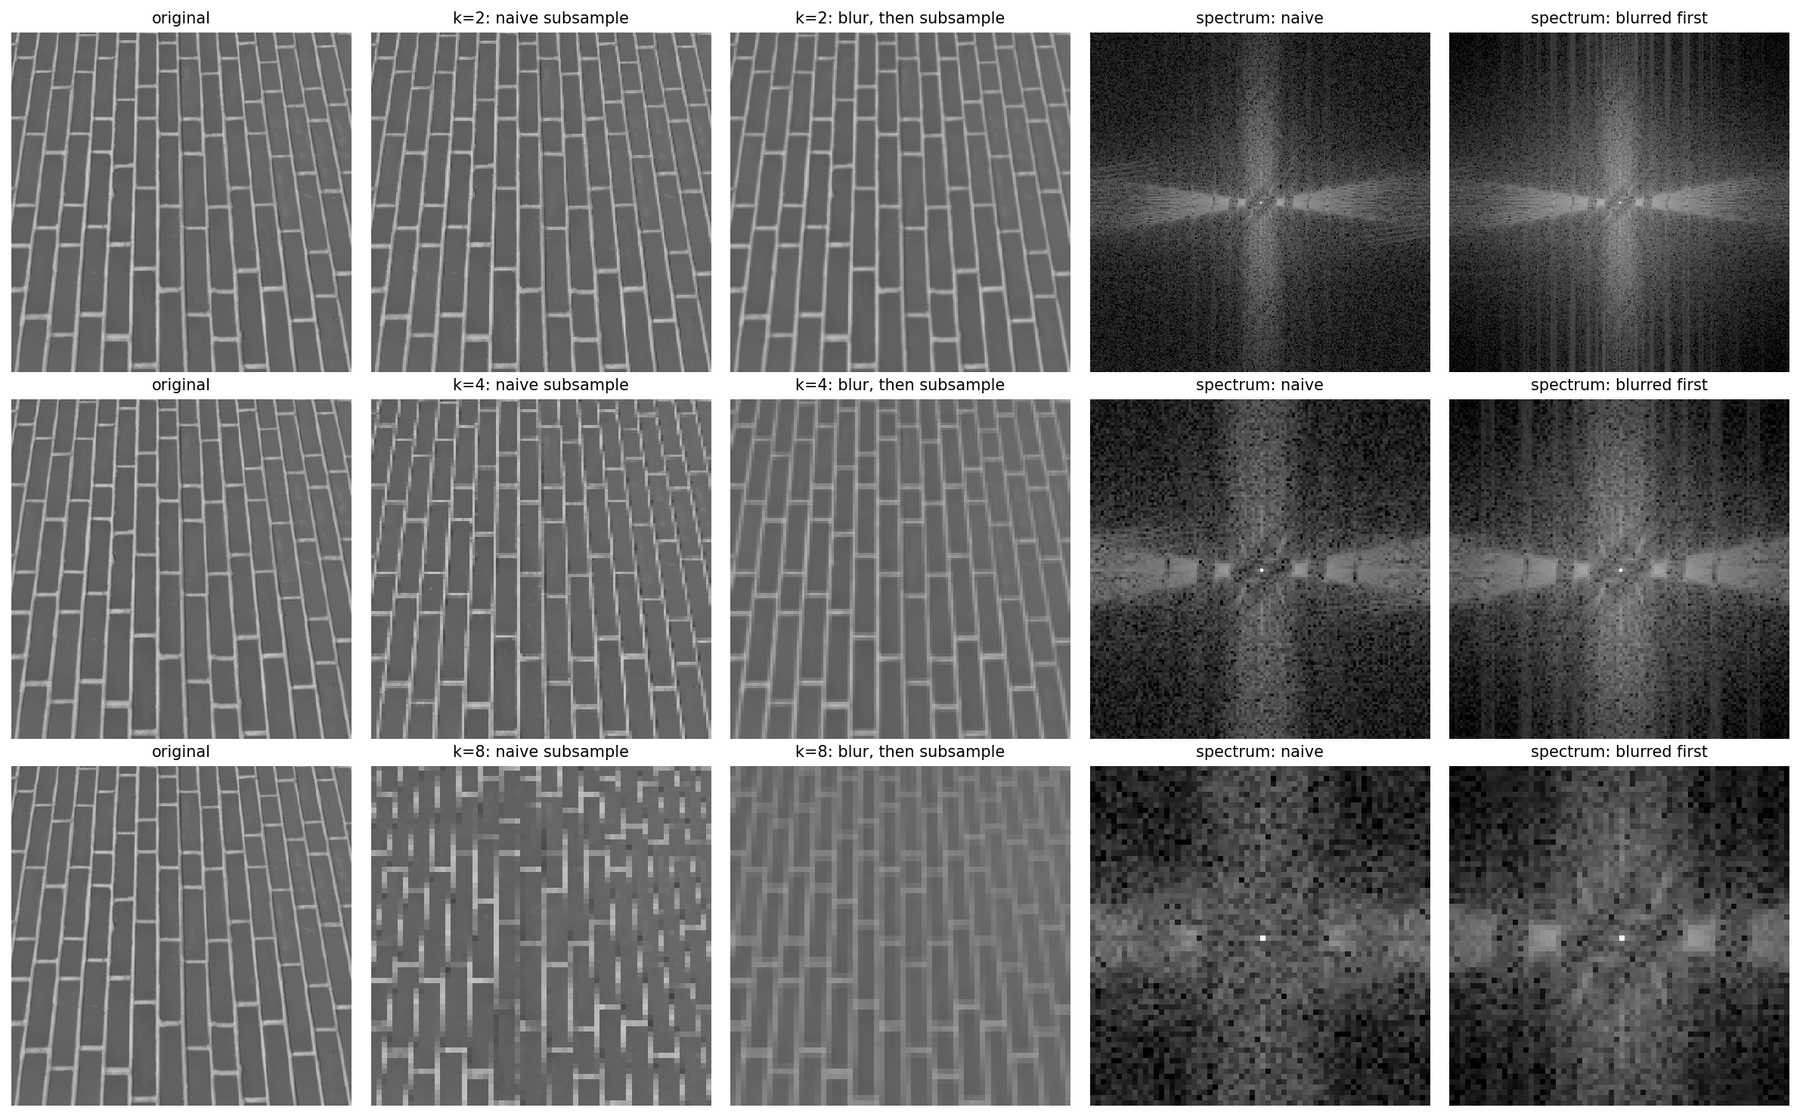
\includegraphics[width=\linewidth]{2_2_brick.png}
  \caption{The same experiment on a brick wall (\texttt{brick.png}).}
\end{figure}

\begin{whybox}
Bricks are a repeating pattern, the natural-image equivalent of the rings. With naive subsampling at $k=4$ the courses and the mortar lines
become irregular, and at $k=8$ the wall is scrambled: bricks of different widths and broken lines that do not exist in the original. Blurring first keeps
a regular grid of bricks, softer but truthful. Its spectrum has energy only near the center, while the naive spectrum is filled out to
the borders: that extra energy is the folded high frequencies.
\end{whybox}

% =====================================================================
\section{Gaussian and Laplacian pyramids (2.3)}
\label{sec:pyr}

\subsection{Implementation}
Both \texttt{reduce} and \texttt{expand} blur with $\frac1{16}[1\,4\,6\,4\,1]$ along $x$ and $y$ (our separable convolution, reflect padding).
\needspace{16\baselineskip}

\begin{lstlisting}
K = outer([1,4,6,4,1], [1,4,6,4,1]) / 256            # separable, rank 1

def reduce(img):                                      # blur, keep every other row/col
    return convolve(img, K, "reflect")[::2, ::2]

def expand(img, out_shape):                           # zeros between pixels, blur, x4
    out = np.zeros(out_shape + img.shape[2:])
    out[::2, ::2] = img                               # top-left of each 2x2 block
    return 4.0 * convolve(out, K, "reflect")          # odd sides: out_shape drops the extra row/col

def laplacian_pyramid(img, levels):
    g = gaussian_pyramid(img, levels)                 # G0 = img, G(i+1) = reduce(G(i))
    return [g[i] - expand(g[i+1], g[i].shape) for i in range(len(g)-1)] + [g[-1]]

def reconstruct(lap):
    img = lap[-1]
    for L in reversed(lap[:-1]):
        img = L + expand(img, L.shape)
    return img
\end{lstlisting}

The test image is the facade photograph ($466\times512$, neither side a power of $2$). Level sizes, with $\lceil n/2\rceil$ at each step:
$466\times512,\ 233\times256,\ 117\times128,\ 59\times64,\ 30\times32,\ 15\times16$.

\begin{figure}[H]
  \centering
  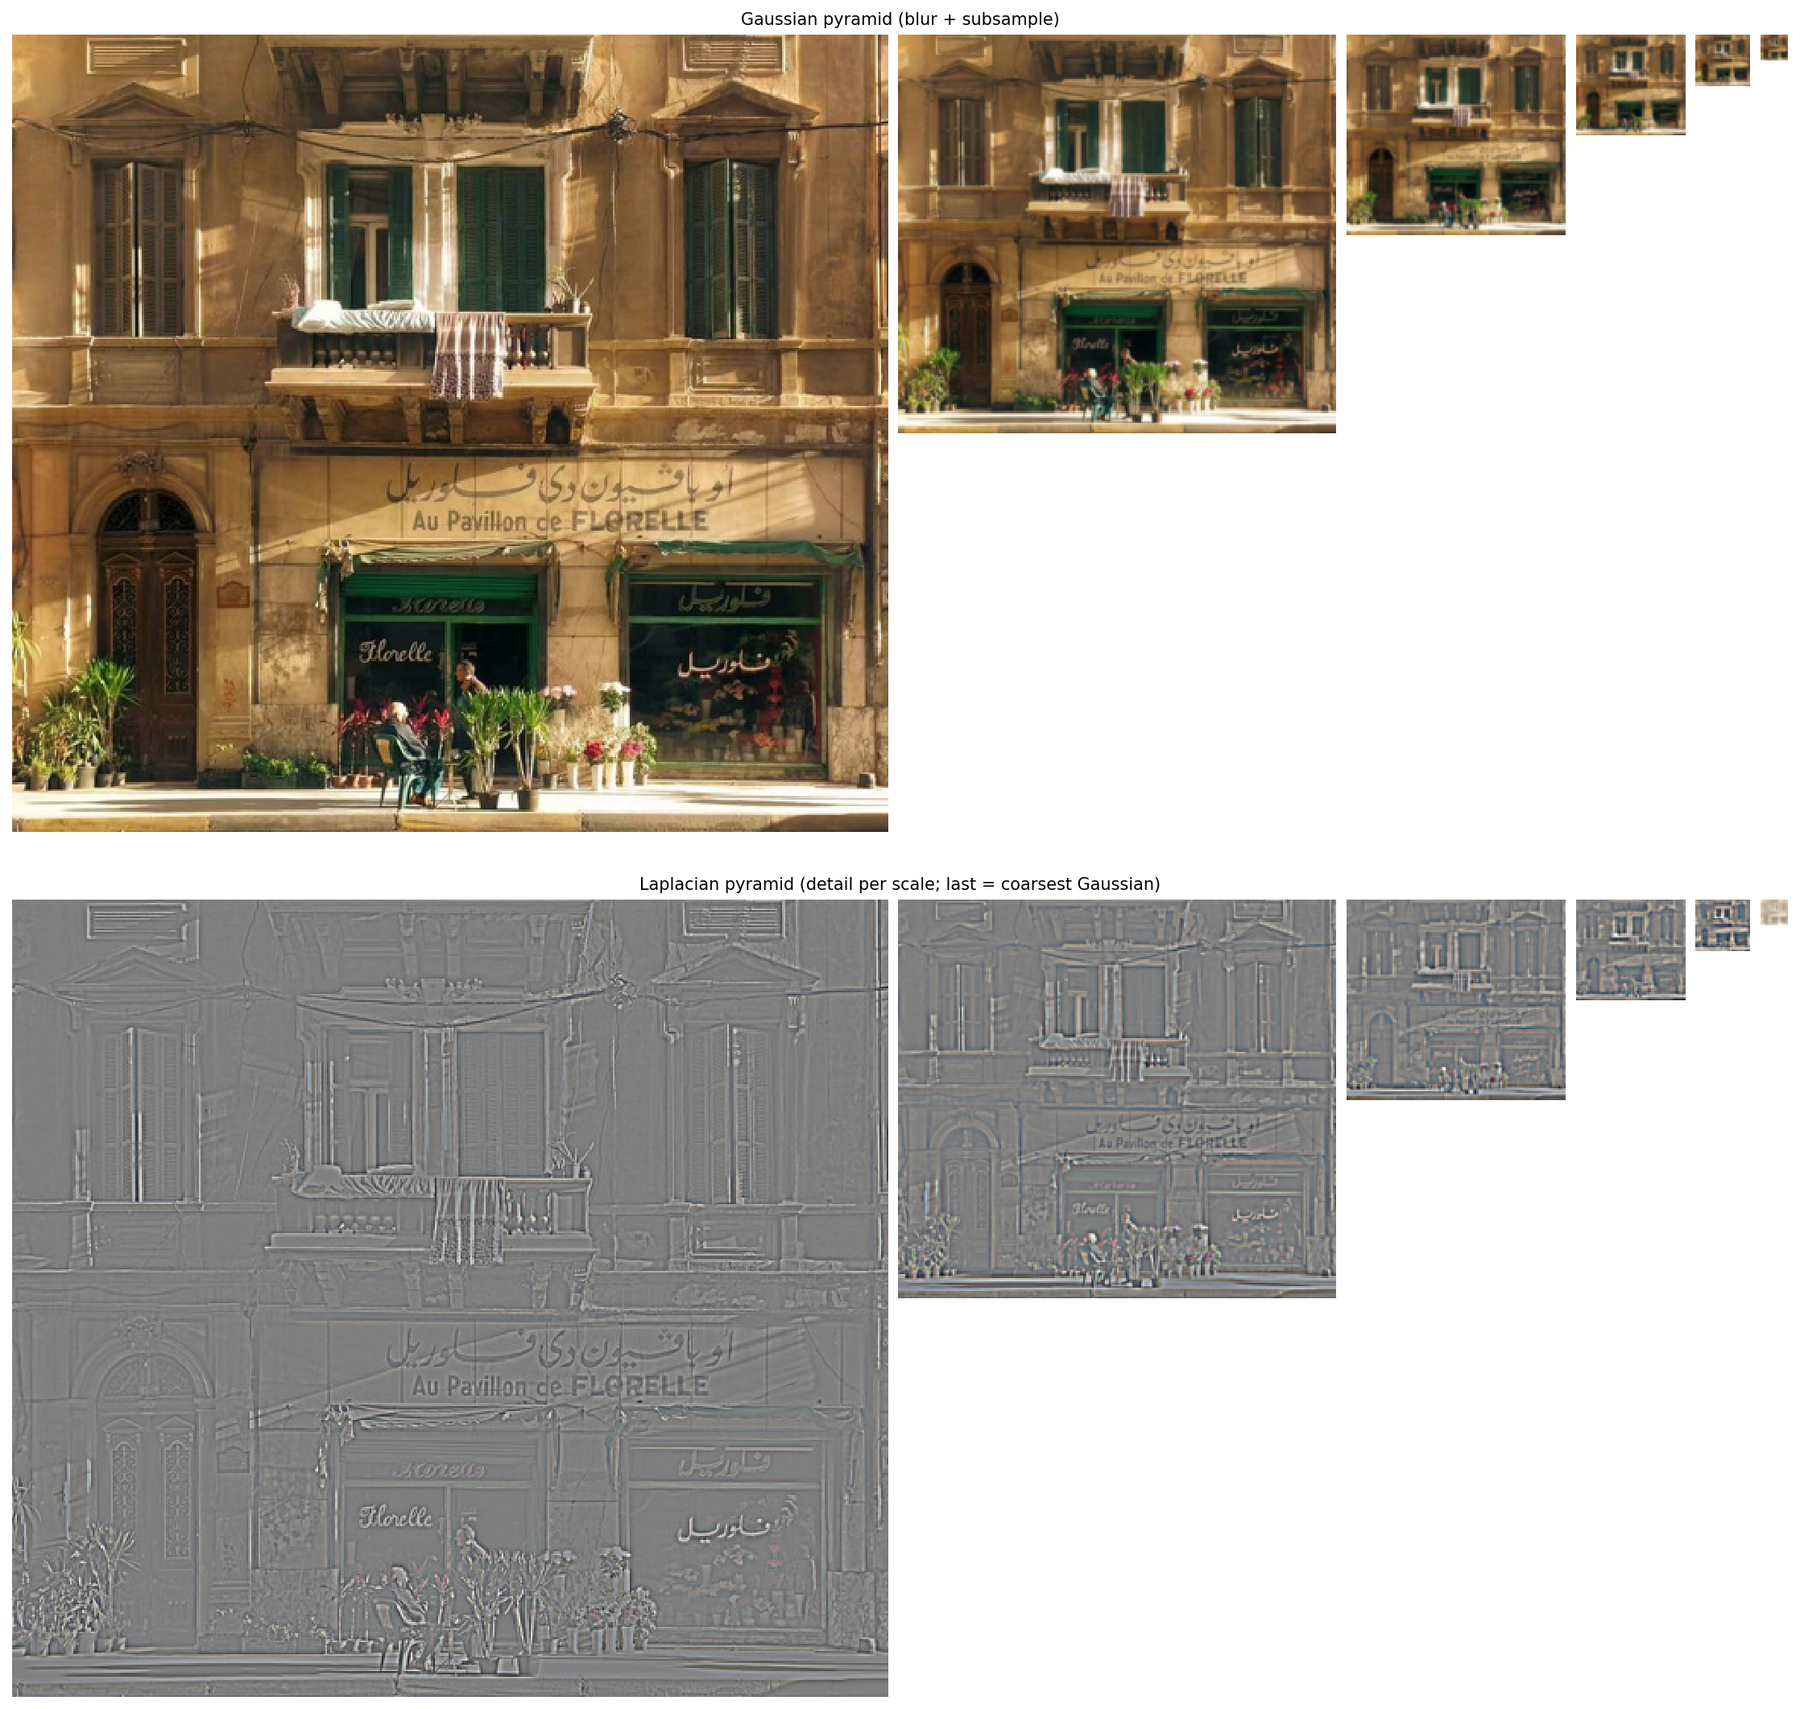
\includegraphics[width=0.95\linewidth]{2_3_pyramids.png}
  \caption{Gaussian pyramid (top) and Laplacian pyramid (bottom, each level stretched to its own contrast, zero = mid-gray); the last Laplacian
  tile is the coarsest Gaussian level.}
\end{figure}

\begin{figure}[H]
  \centering
  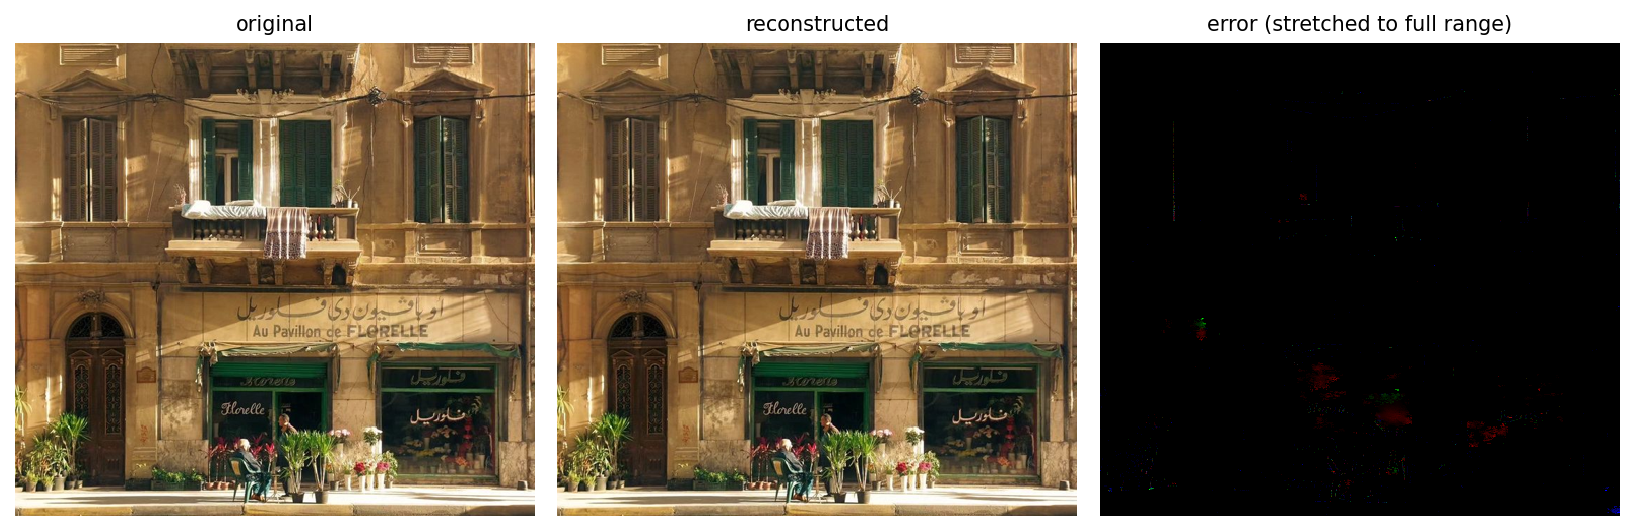
\includegraphics[width=\linewidth]{2_3_reconstruction.png}
  \caption{Original, image rebuilt from the Laplacian pyramid, and the absolute error stretched to the full range. The maximum error is
  $1.11\times10^{-16}$.}
\end{figure}

\begin{whybox}
The stretched error image looks like sparse colored specks, not like an edge map. That is the point: the largest difference is $10^{-16}$, about half of
double-precision machine epsilon ($2.2\times10^{-16}$), so what we see is rounding noise magnified to full contrast, not a structural error.
\end{whybox}

\begin{figure}[H]
  \centering
  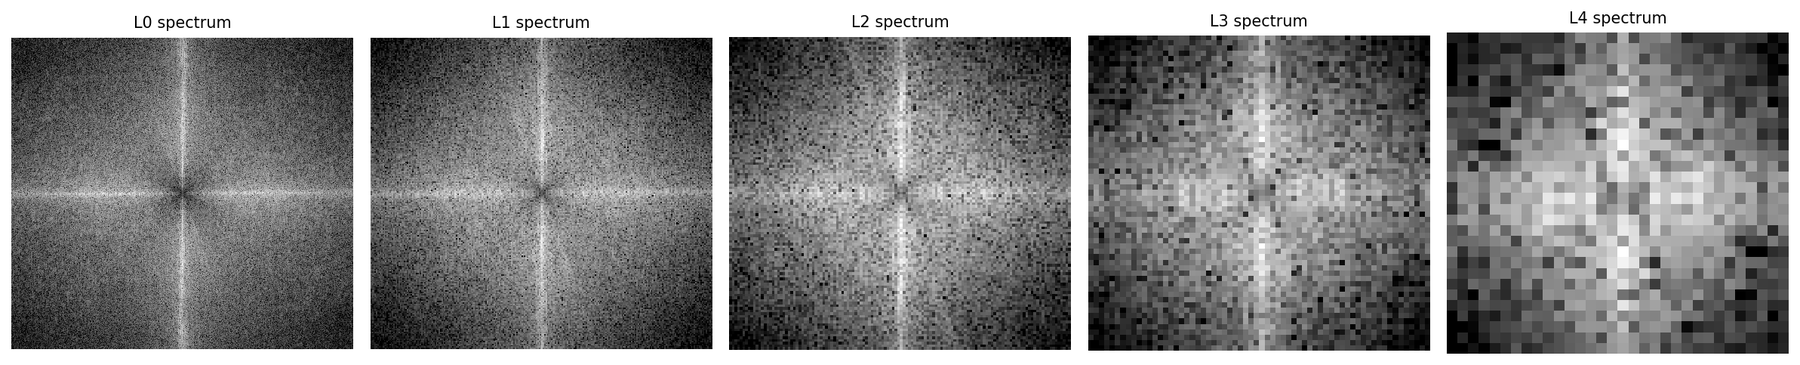
\includegraphics[width=\linewidth]{2_3_band_spectra.png}
  \caption{Spectrum of Laplacian levels $L_0$ to $L_4$ (each on its own grid). Every level has a dark center, because the low frequencies are exactly
  what was subtracted.}
\end{figure}

\subsection{Why the rebuild is exact, and why the Lecture 3 version is not}

\begin{answerbox}
\textbf{Exactness.} Each Laplacian level is \emph{defined} as
$L_i=G_i-\text{expand}(G_{i+1})$, and the rebuild computes $G_i=L_i+\text{expand}(G_{i+1})$ with the \emph{same}
\texttt{expand} applied to the \emph{same} $G_{i+1}$ (which the rebuild has already recovered). It is the identity
$(G_i-E)+E=G_i$ at every level, starting from the stored coarsest level $G_{\text{last}}$, so nothing is approximated; the only error is floating-point
rounding. Subsampling really throws information away, but that information is exactly what is stored in $L_i$: $L_i$ is the residual of the
\emph{prediction} $\text{expand}(G_{i+1})$.

\textbf{The Lecture 3 version is not exact.} There each level is the image minus its \emph{blur} at the same size,
$G_i-\text{blur}(G_i)$. That works as long as every level keeps the full resolution, so the pieces telescope. As soon as the
levels are subsampled to save memory, the rebuild no longer has $\text{blur}(G_i)$: it has only the small image, and
$\text{expand}(\text{reduce}(G_i))\neq\text{blur}(G_i)$ (the former is an interpolation of a subsampled signal). The stored detail was computed against a different prediction than the one used to rebuild, so the sum does not return $G_i$.
\end{answerbox}

\subsection{Total size of the Gaussian pyramid}

\begin{answerbox}
\textbf{The Gaussian pyramid holds $\boldsymbol{\tfrac43}$ of the pixels of the image.}
Each level has a quarter of the pixels of the one before, so the total is
\begin{equation}
  1+\tfrac14+\tfrac1{16}+\cdots=\sum_{i\ge0}4^{-i}=\frac{1}{1-1/4}=\frac43\approx1.333 .
\end{equation}
Our six levels measure $1.3336$ (printed by the notebook). The exact partial sum of six terms is $1.3330$, and the measured value is slightly larger
because odd sizes are rounded \emph{up} ($\lceil n/2\rceil$), which is also why the rebuild works for odd sides.
\end{answerbox}

\begin{whybox}
The $33\%$ overhead is the price of keeping every scale. The Laplacian pyramid has the same number of coefficients, so it is not a compression by itself;
what makes it useful is that most of its values are near zero (flat regions have no detail), so it is sparse and compresses well. The factor $4$ in
\texttt{expand} has a simple reason: three of every four pixels of the zero-padded grid are $0$, and the kernel sums to $1$, so the blur would
divide brightness by $4$ ($2$ per axis). Multiplying by $4$ puts it back, and we checked that a flat image stays exactly flat through \texttt{expand},
including at odd sizes and at the borders.
\end{whybox}

% =====================================================================
\section{Multiresolution blending (2.4)}

\subsection{Method}
Given two images $A$, $B$ and a mask $M$ ($1$ where we want $A$), build the Laplacian pyramids $L^A_i$, $L^B_i$ and the Gaussian
pyramid $M_i$ of the mask. At every level the bands are mixed with that level's mask and the result is collapsed exactly as in 2.3:
\begin{equation}
  L^{H}_i \;=\; M_i\,L^A_i + (1-M_i)\,L^B_i ,\qquad H=\text{reconstruct}\bigl(L^H\bigr).
\end{equation}
The mask given to the function is sharp; its Gaussian pyramid does the softening. Because each level's mask has been
reduced $i$ times with a unit-variance kernel, the mask at level $i$ is blurred by $\sigma_i\approx\sqrt{(4^i-1)/3}$ original pixels:
\begin{center}
\small
\begin{tabular}{@{}lcccccc@{}}
\toprule
level $i$ & 0 & 1 & 2 & 3 & 4 & 5\\
\midrule
$\sigma_i$ (original pixels) & 0 & 1.0 & 2.2 & 4.6 & 9.2 & 18.5\\
\bottomrule
\end{tabular}
\end{center}
Fine levels switch images almost abruptly and coarse levels over tens of pixels.

\subsection{Blend 1: the oraple}
Mask: the left half white, built in code (\texttt{vertical\_mask}: ones in the left $50\%$ of the columns, zeros elsewhere). Both
images are $512\times512$. \textbf{Levels used: 6.}
Besides the hard cut required by the handout we also show a single-scale feather (the same mask blurred once with
$\sigma=15$), to show that blurring the mask is not enough on its own.

\begin{figure}[H]
  \centering
  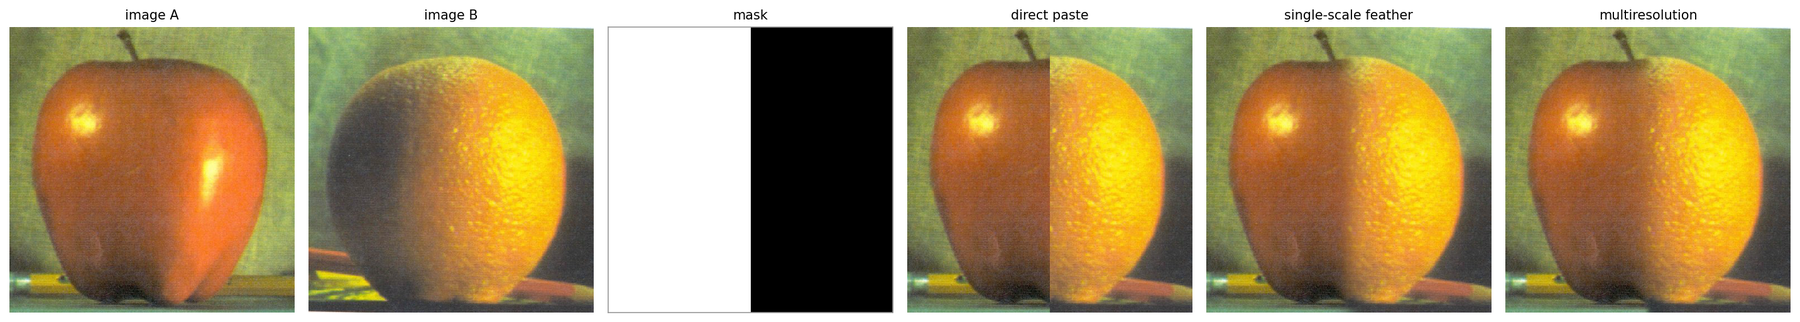
\includegraphics[width=\linewidth]{2_4_oraple_comparison.png}
  \caption{Apple, orange, mask, hard cut, single-scale feather and multiresolution blend (6 levels).}
\end{figure}

\begin{figure}[H]
  \centering
  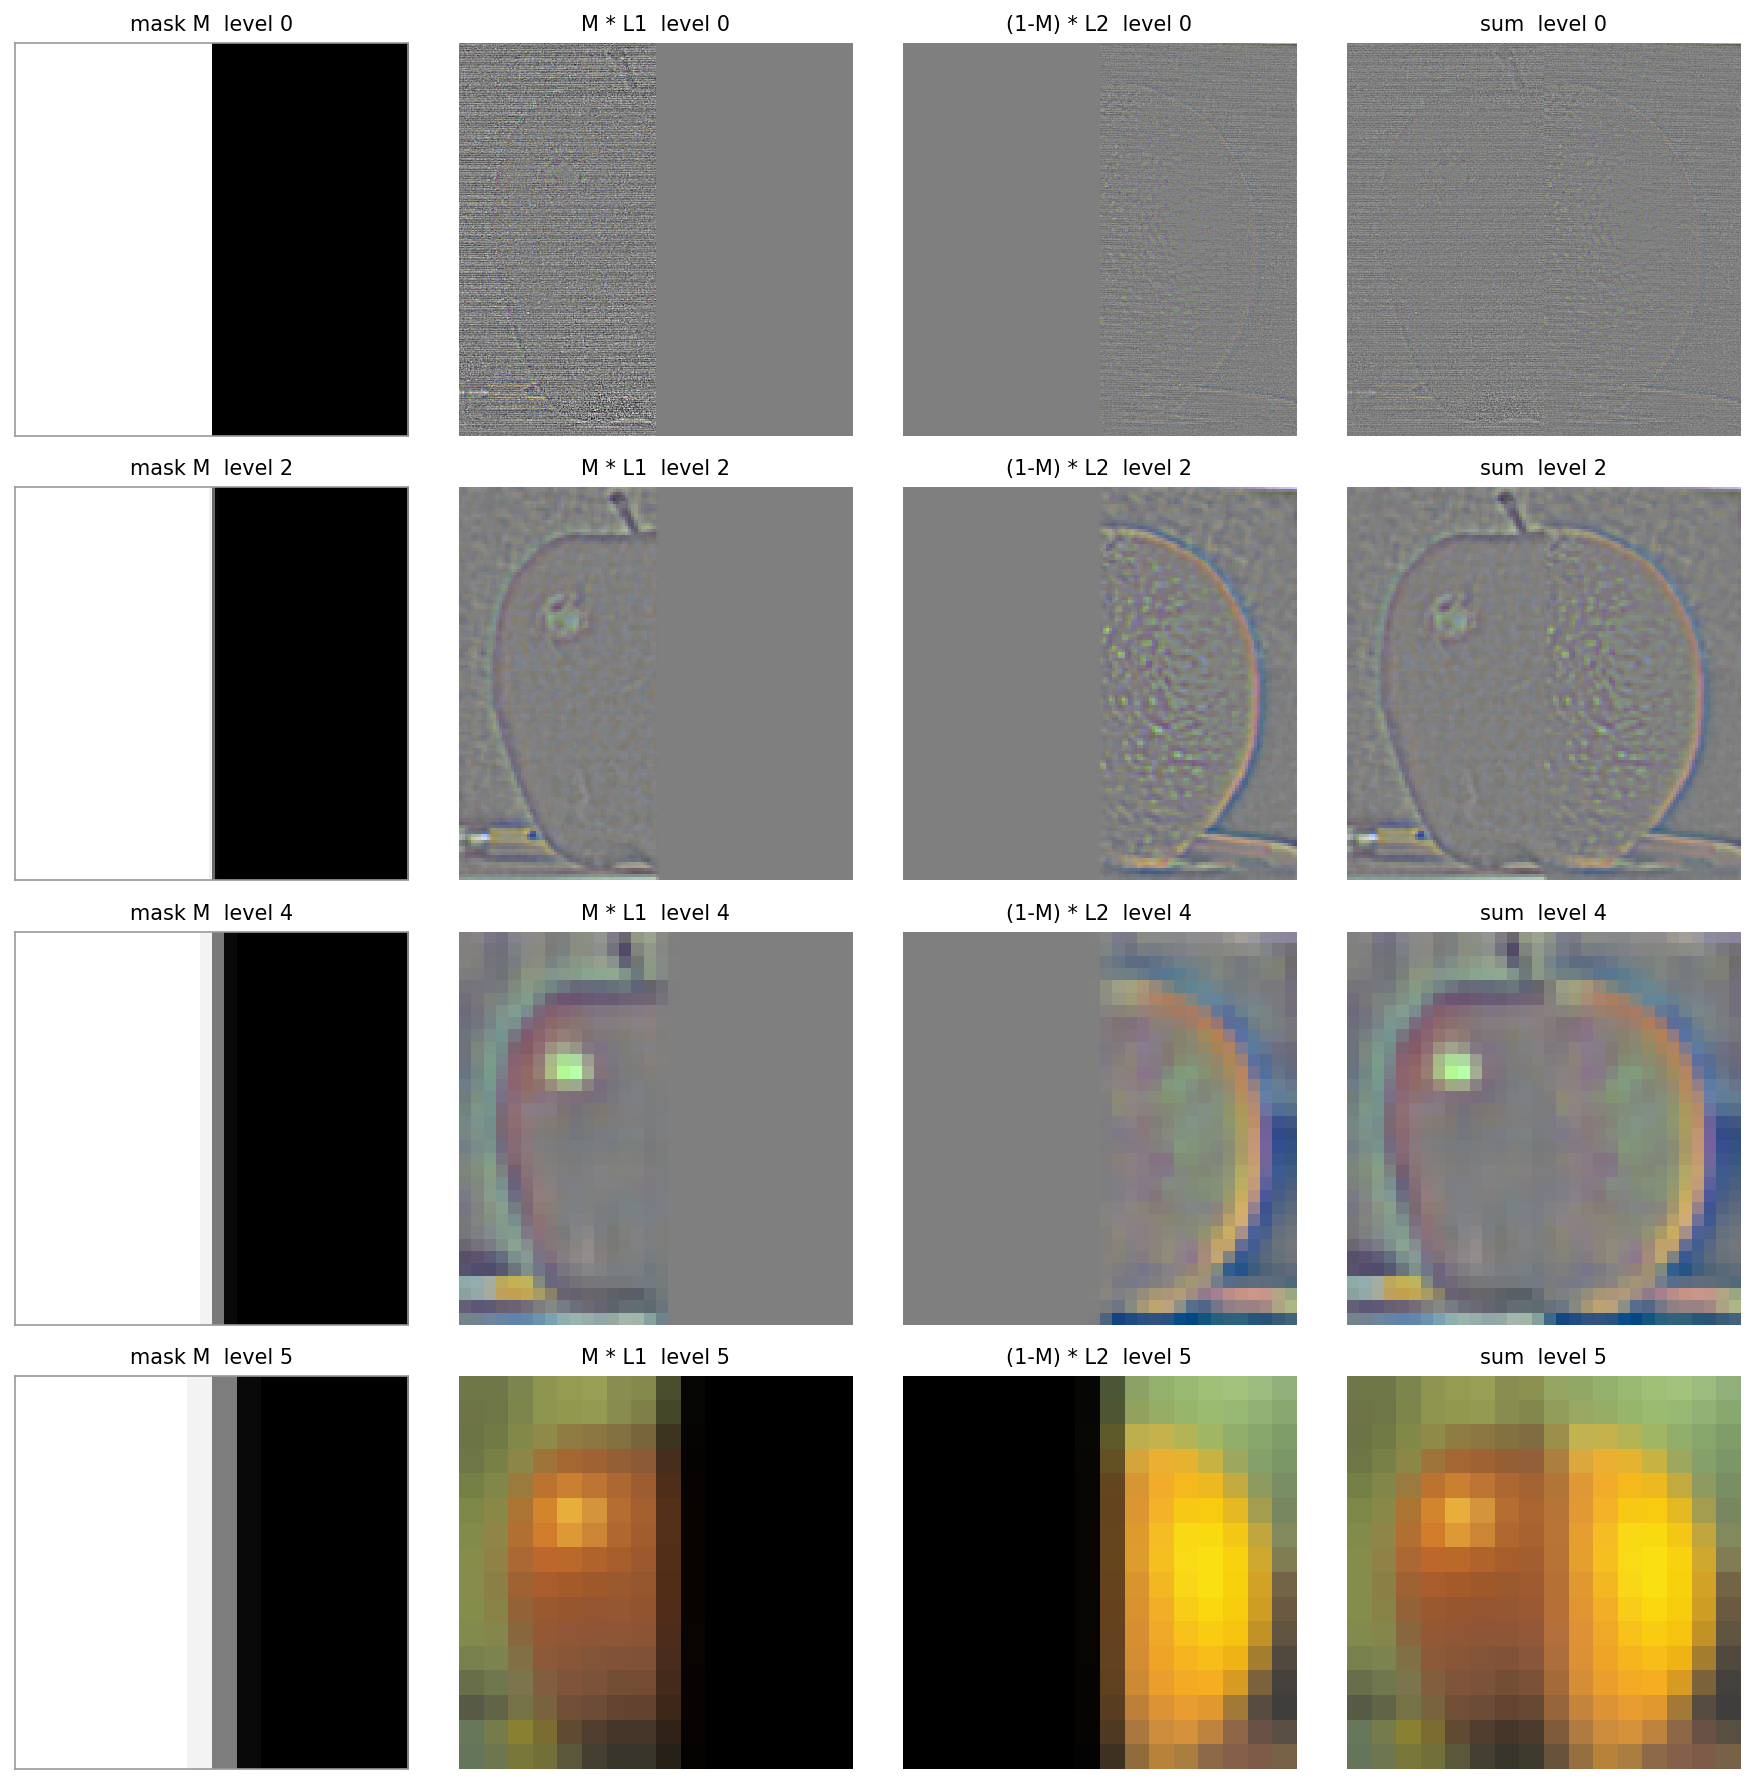
\includegraphics[width=0.9\linewidth]{2_4_oraple_levels.png}
  \caption{Level by level (levels 0, 2, 4, 5): the mask $M_i$, $M_i L^A_i$, $(1-M_i)L^B_i$, and their sum, which is the blended level.
  Levels 0, 2 and 4 are signed (zero = mid-gray); the last level is the coarsest Gaussian and is shown as is.}
  \label{fig:oraple_levels}
\end{figure}

\begin{answerbox}
\textbf{Why blending band by band hides the seam that the hard cut shows.}
An image is a sum of bands, and each band needs a different transition width to look natural.
\emph{Coarse bands} (overall color and brightness) change gently inside each image, so a step in them is conspicuous: they must be
mixed over a \emph{wide} region, comparable to their own wavelength. \emph{Fine bands} (the orange's peel, the apple's smooth skin) must be mixed over
a \emph{narrow} region, because mixing them over a wide one superimposes two different textures: a ghost, the double exposure of the feather result. A hard cut uses a
transition of one pixel for every band, so the coarse bands jump from apple-red to orange-yellow at the cut, and the eye sees that jump as the seam.
The mask's Gaussian pyramid gives each band its own width for free: Figure~\ref{fig:oraple_levels} shows the mask nearly sharp
at level 0 and spread over tens of pixels at level 5.
\end{answerbox}

\begin{whybox}
\textbf{What the level figure shows.} At level 0 ($\sigma_0=0$) the mask is a hard edge, and yet there is no visible seam, because that band holds
only the finest texture (details of a pixel or two), and a texture is allowed to change abruptly. At level 5 the mask is blurred by about $18$ pixels (a transition roughly $45$ pixels wide), and the
color of the apple fades into the color of the orange gradually. The single-scale feather
cannot do both: with $\sigma=15$ its transition is wide enough to hide neither the fine texture change nor the color step, and a soft vertical band is
still visible in the result.
\end{whybox}

\subsection{Blend 2: a face on a pumpkin}

\textbf{Inputs.} A pumpkin photograph ($563\times1000$) and a frontal portrait ($595\times1000$), both resized so that the longer side is $1000$ pixels, as
the handout recommends.

\textbf{Alignment} (\texttt{align\_images.py}, two points on each image). The two eye centers of the portrait, $(216,331)$ and $(381,331)$, are sent to
$(213,425)$ and $(341,425)$ on the pumpkin's body. Both pairs are horizontal, so the transform is a pure shrink by $0.776$ and a shift (no rotation); the
shrink makes the face fit on the pumpkin.

\textbf{Mask.} A $24$-point polygon traced on the \emph{portrait} around the skin of the face (hairline to chin, between the ears; hair, ears and neck are
left out). The polygon is mapped onto the pumpkin with the \emph{same} two-point transform that moves the pixels, so mask and image cannot drift apart,
and it is filled with \texttt{cv2.fillPoly}. The result is an irregular, hard-edged shape of $268\times366$ pixels ($14.9\%$ of the image).
\textbf{Levels used: 5} (the image allows $7$).

\begin{figure}[H]
  \centering
  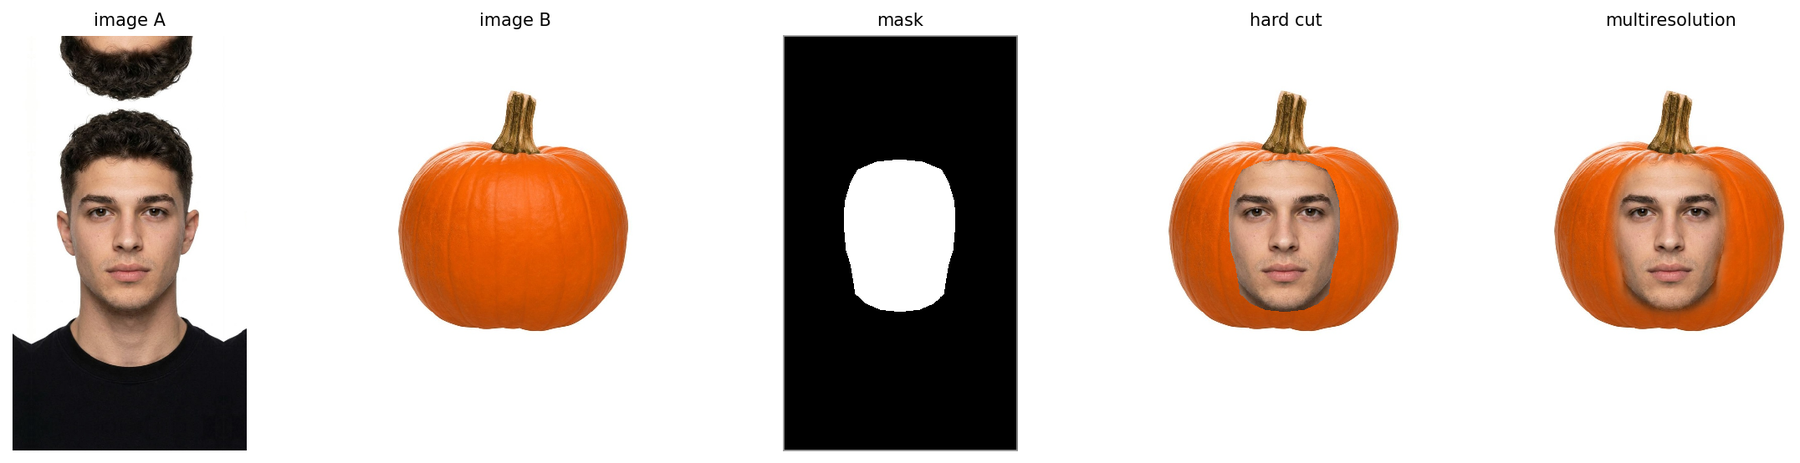
\includegraphics[width=\linewidth]{2_4_face_pumpkin_comparison.png}
  \caption{Image A (the portrait, aligned onto the pumpkin's frame), image B (the pumpkin), the mask, the hard cut and the multiresolution blend (5 levels).}
\end{figure}

\begin{figure}[H]
  \centering
  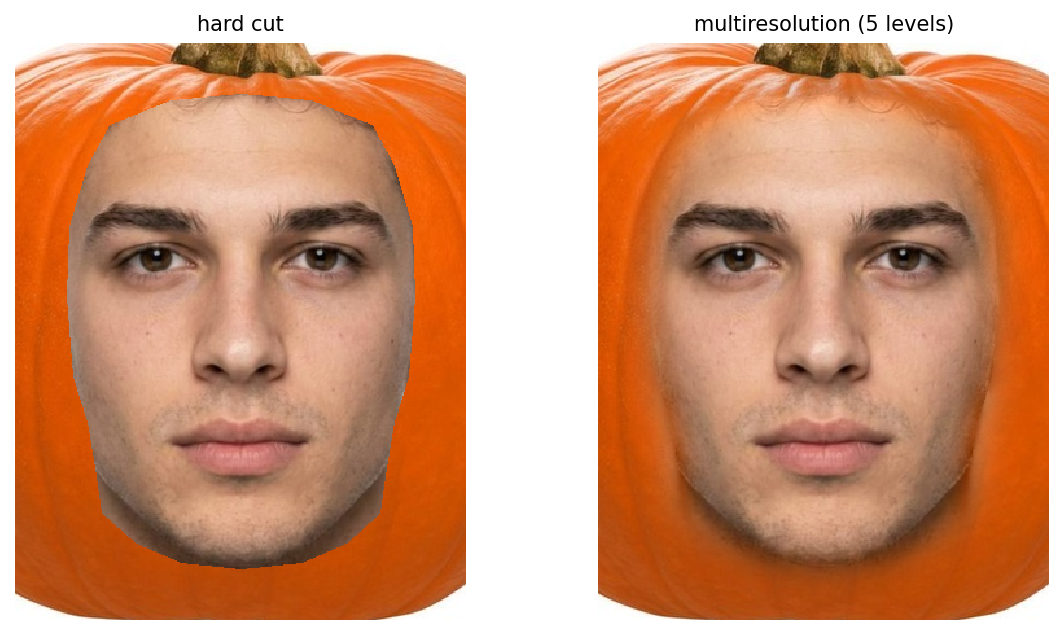
\includegraphics[width=0.8\linewidth]{2_4_face_pumpkin_zoom.png}
  \caption{The same result zoomed around the face: hard cut (left) and multiresolution blend (right).}
\end{figure}

\begin{whybox}
\textbf{Hard cut.} The face looks like a sticker: its pale skin stops at a one-pixel outline against the saturated, strongly textured orange, and the eye
reads that outline as an edge.
\textbf{Multiresolution.} The eyes, brows and lips are fine and mid-frequency structure that exists only in the portrait, and inside the polygon the mask is $1$ at \emph{every}
level, so they stay as crisp as in the original. Only near the outline do the coarse bands (overall color and brightness) fade into the pumpkin's, so the rim of the face takes on a
little orange, as if lit by the pumpkin, instead of ending in a line.
\textbf{What it does not do.} The interior keeps the portrait's own color and lighting (frontal and pale, against a pumpkin lit from the upper left), because inside the mask only the portrait's bands are used.
Blending hides the \emph{seam}; it does not make two differently lit objects consistent.
\end{whybox}

\subsection{Blend 3: an eye on the moon}

\textbf{Inputs.} A macro photograph of an eye ($736\times981$) and a night photograph of the full moon ($667\times1000$, resized as above). The moon's disc has its center
near $(336,450)$ and a radius of about $214$ pixels.

\textbf{Alignment.} The inner and the outer corner of the eye, $(95,635)$ and $(700,583)$, are sent to $(170,464)$ and $(502,436)$, two points across the moon's disc.
The corner-to-corner line has the same tilt in both images, so the rotation is $0.1^\circ$; the scale is $0.549$, which makes the eye about $330$ pixels wide, roughly $78\%$ of the moon's diameter.

\textbf{Mask.} An $18$-point almond-shaped polygon traced on the eye photograph along the tips of the upper lashes and the lower lid, mapped onto the moon through the same
transform and filled with \texttt{cv2.fillPoly}: $327\times170$ pixels, $5.8\%$ of the image. \textbf{Levels used: 5} (the image allows $7$).

\begin{figure}[H]
  \centering
  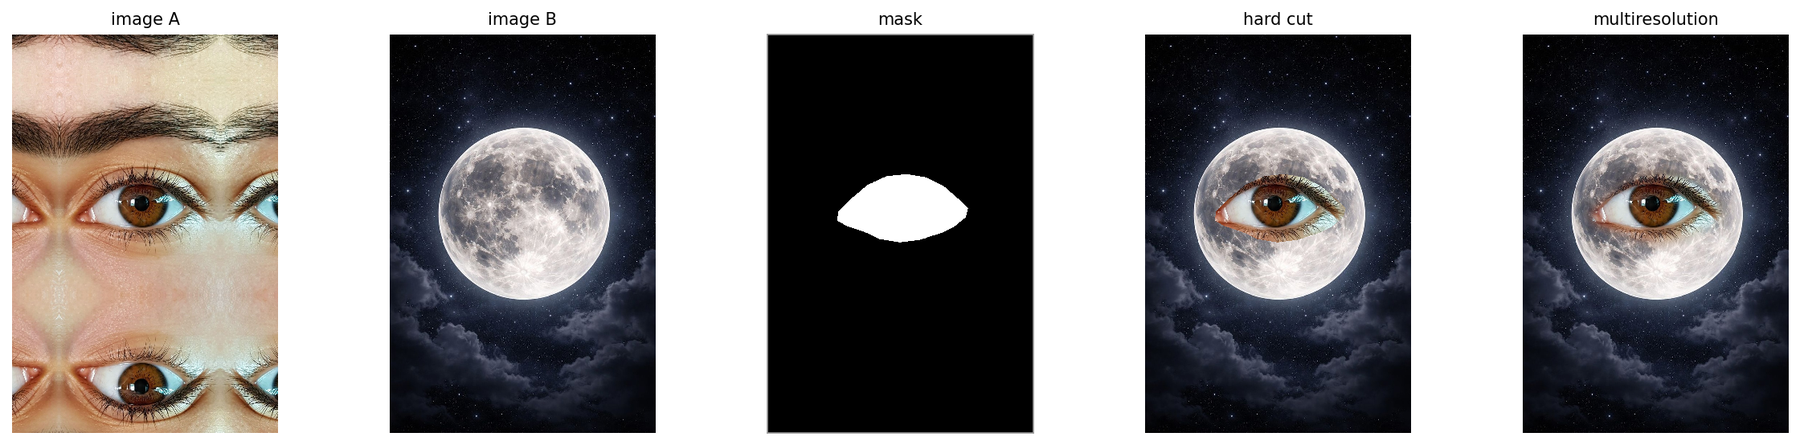
\includegraphics[width=\linewidth]{2_4_eye_moon_comparison.png}
  \caption{Image A (the eye, aligned onto the moon's frame), image B (the moon), the mask, the hard cut and the multiresolution blend (5 levels).}
\end{figure}

\begin{figure}[H]
  \centering
  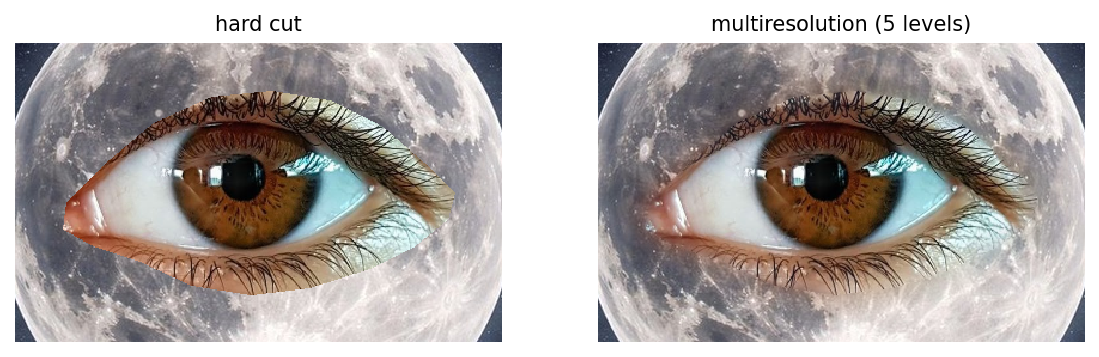
\includegraphics[width=\linewidth]{2_4_eye_moon_zoom.png}
  \caption{Zoom on the eye: hard cut (left) and multiresolution blend (right).}
\end{figure}

\begin{whybox}
In the hard cut the pasted region keeps a visible rim of pinkish eyelid skin that ends abruptly on the gray moon. In the blend that rim melts into the surface:
the lashes and the iris remain sharp, while the skin tone fades out over a few tens of pixels. Because the eye is warm and dark and the moon is cool and light, almost all of the
difference between the two images is in the coarse bands, which is exactly where a wide transition is needed.
\end{whybox}

\paragraph{Favorite: the eye on the moon, level by level.}
Figure~\ref{fig:eye_levels} shows four of the five levels (0, 1, 3, 4).

\begin{figure}[H]
  \centering
  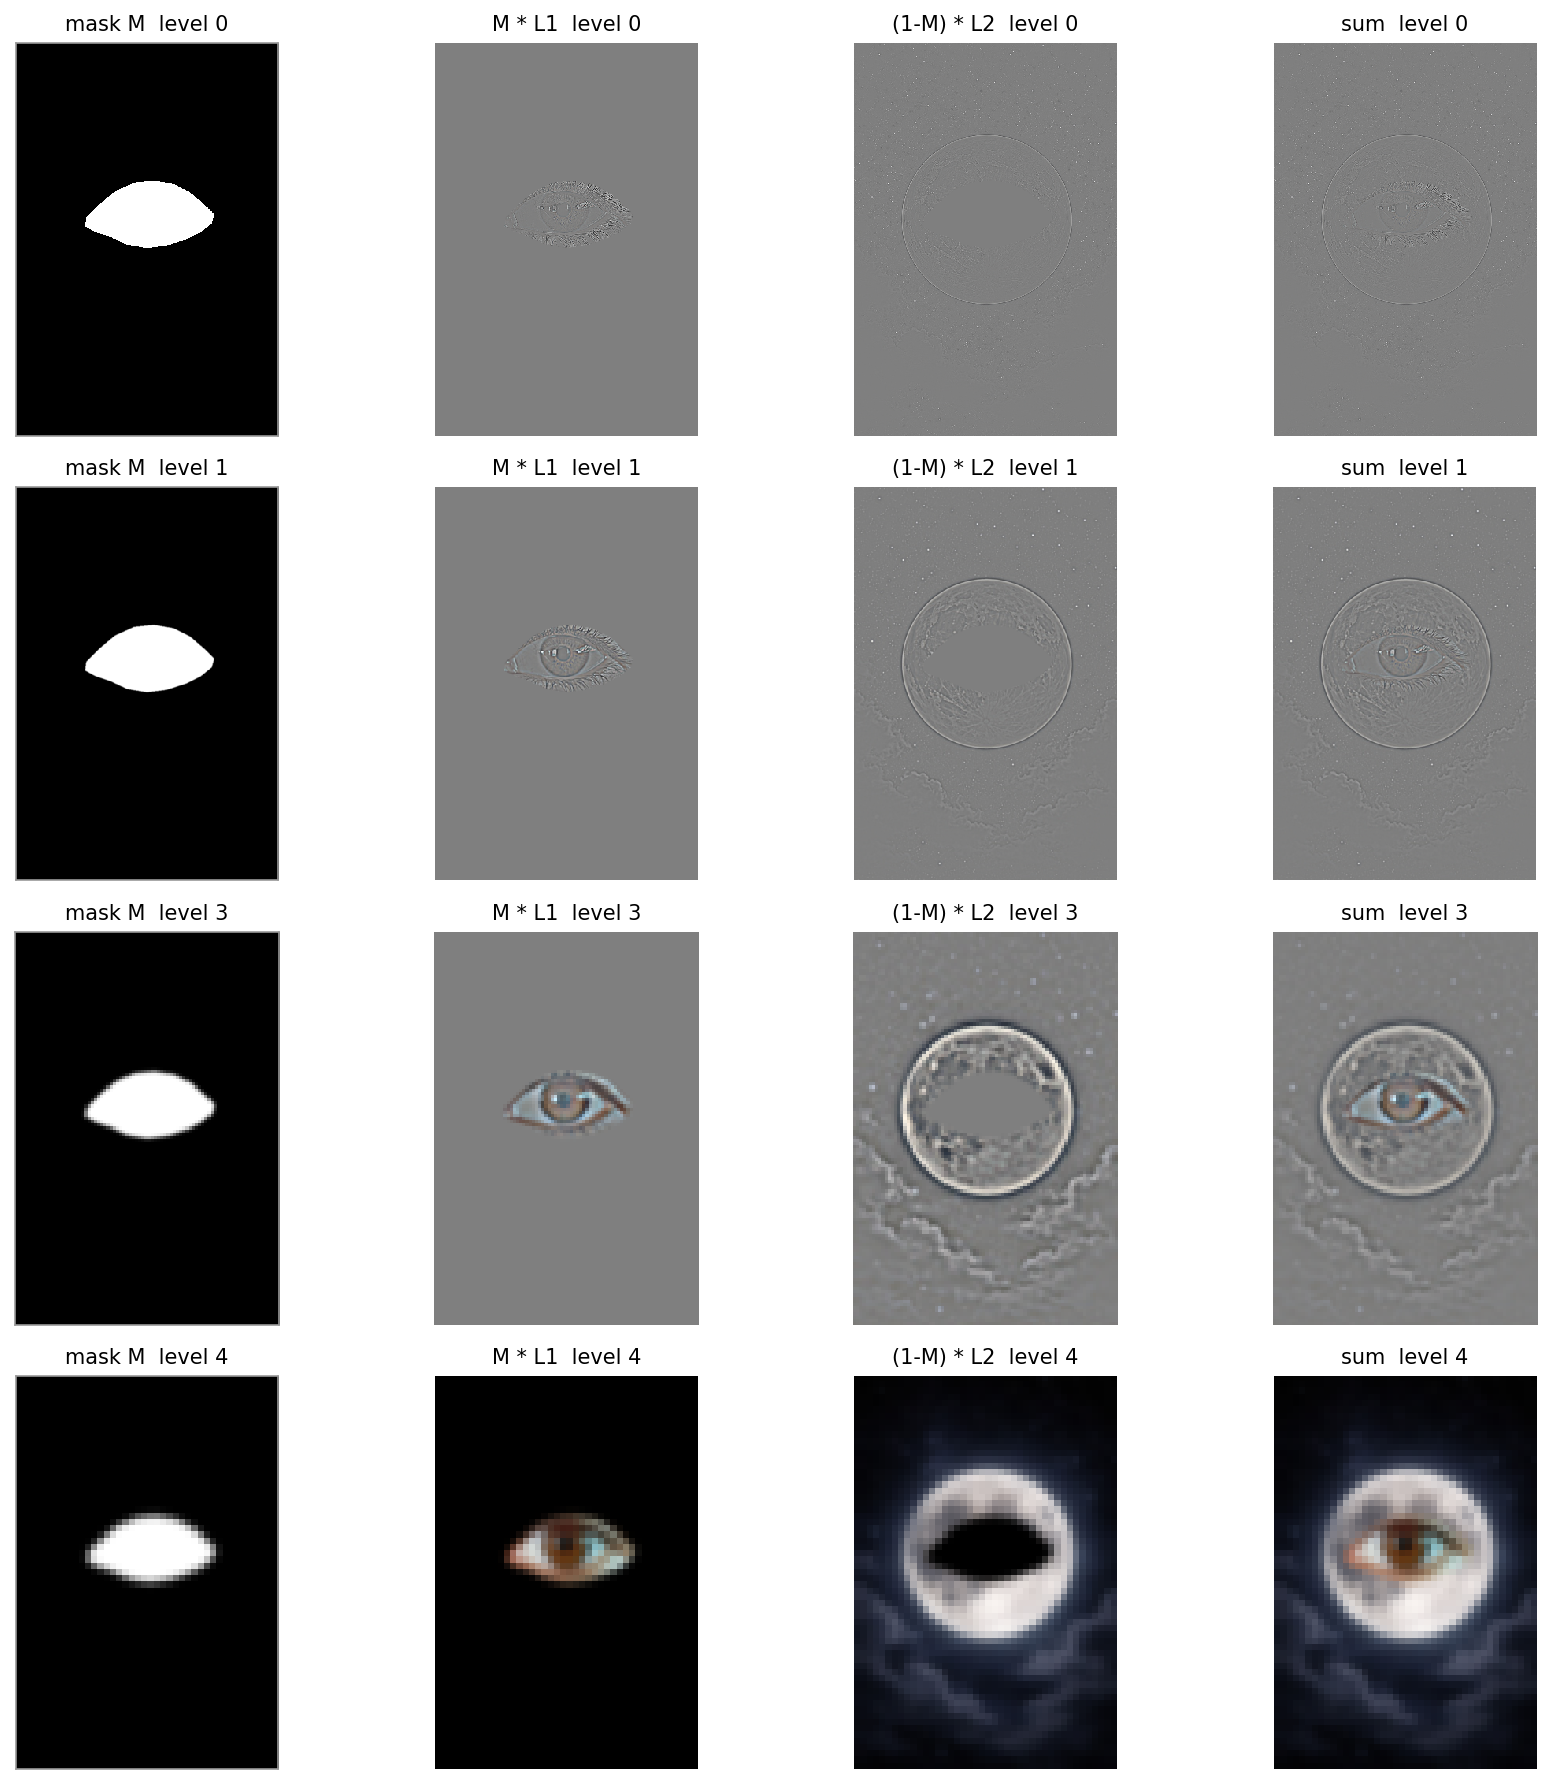
\includegraphics[width=0.78\linewidth]{2_4_eye_moon_levels.png}
  \caption{Eye on the moon, levels 0, 1, 3 and 4: the mask $M_i$, $M_iL^A_i$ (the eye's contribution), $(1-M_i)L^B_i$ (the moon's contribution) and their sum.
  Levels 0, 1 and 3 are signed (zero = mid-gray); level 4 is the coarsest Gaussian and is shown as is.}
  \label{fig:eye_levels}
\end{figure}

\begin{whybox}
\textbf{Reading the figure.} At levels 0 and 1 the eye contributes only thin lashes and edges, and the moon contributes its finest detail (stars, the thin
bright rim of the limb); the mask is almost a hard edge, which is harmless because these bands carry no large-scale color. At level 3 the eye appears as soft colored shapes (iris, pinkish corner,
white of the eye) and the moon's band has a hole exactly where the mask is $1$; the two fill each other, and their sum is continuous. At level 4, the coarsest, the hole in the moon has a soft edge
(the mask is blurred by about $9$ pixels), so the moon's glow wraps around the eye gradually. The sum of the two at every level is already the final
band, which is why the rebuild shows no seam.
\end{whybox}

\subsection{How many levels?}

\begin{figure}[H]
  \centering
  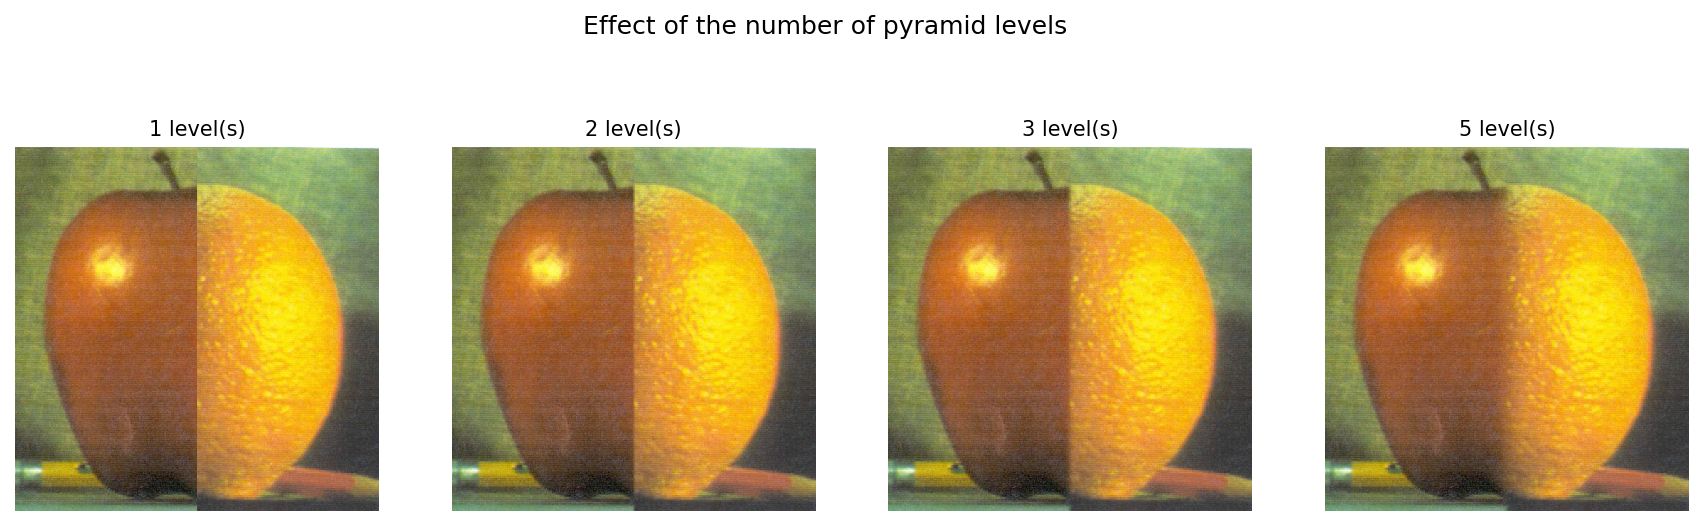
\includegraphics[width=\linewidth]{2_4_levels_sweep.png}
  \caption{Oraple with $1$, $2$, $3$ and $5$ pyramid levels.}
\end{figure}

\begin{figure}[H]
  \centering
  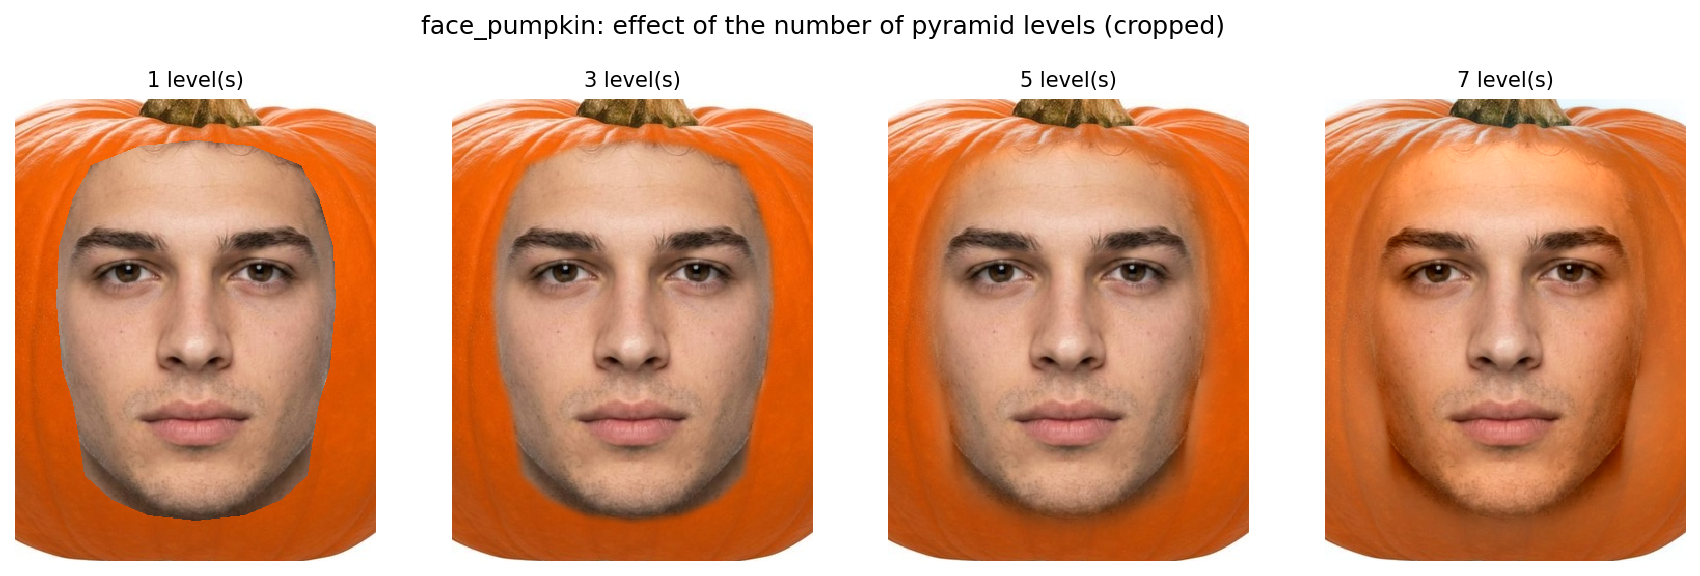
\includegraphics[width=\linewidth]{2_4_face_pumpkin_levels_sweep.png}
  \caption{Face on the pumpkin with $1$, $3$, $5$ and $7$ levels (cropped around the face).}
  \label{fig:face_sweep}
\end{figure}

\begin{figure}[H]
  \centering
  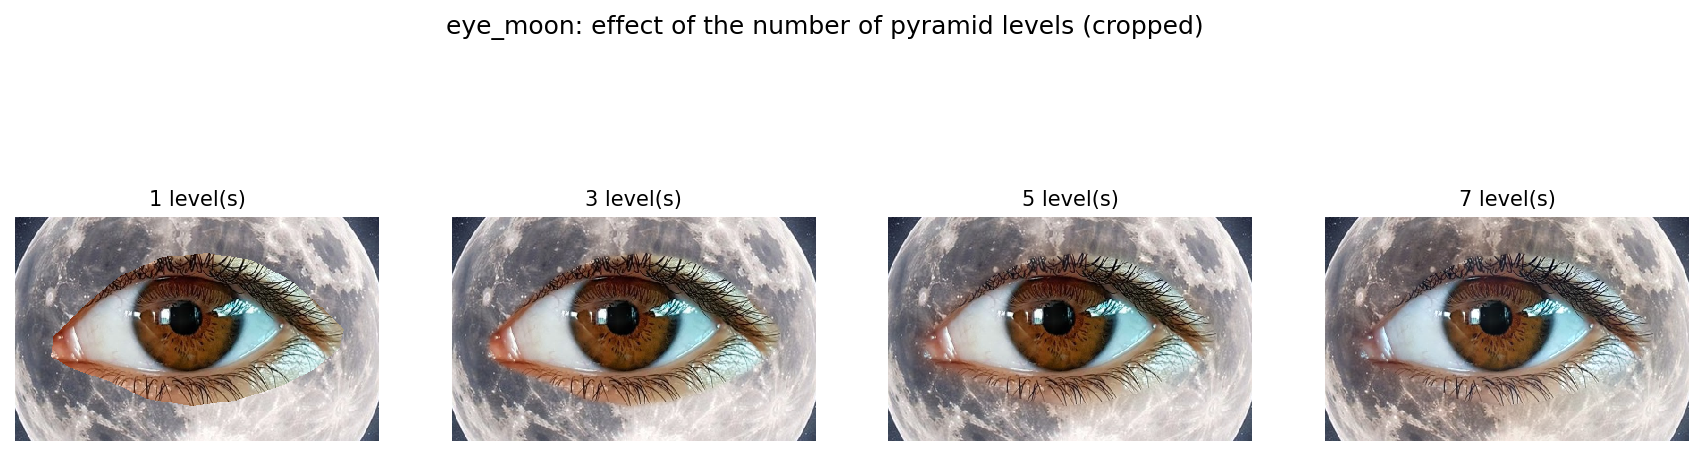
\includegraphics[width=\linewidth]{2_4_eye_moon_levels_sweep.png}
  \caption{Eye on the moon with $1$, $3$, $5$ and $7$ levels (cropped around the eye).}
\end{figure}

\clearpage
\begin{answerbox}
\textbf{Levels used.} Oraple: $6$. Face on the pumpkin: $5$. Eye on the moon: $5$.

\textbf{Too few levels leave the seam.} One level is the hard cut, since there is no pyramid and only the sharp mask is used. With $2$ or $3$ levels the widest transition is only a few pixels:
the oraple still shows a step in color, the face still has a clear outline, and the eye still has its rim of skin. The seam is gone at $5$ levels (we did not render $4$).

\textbf{Too many levels wash out the pasted object.} The widest transition grows quickly: the mask at the last level of a $L$-level pyramid is blurred by $\sigma_{L-1}$, which is
$9.2$ pixels for $5$ levels, $18.5$ for $6$ and $36.9$ for $7$. At $7$ levels the coarsest bands of the face are mixed over about $\pm2\sigma_6\approx\pm74$ pixels
from the outline, and the face's half-width is only $134$ pixels. Figure~\ref{fig:face_sweep} shows the result: the cheeks and forehead take on the pumpkin's orange and the central strip (nose, mouth) mostly keeps
its own color. The eye on the moon is affected less visibly in our render, but its half-height of $85$ pixels is of the same order as the transition at $7$ levels, so the same risk applies.
\end{answerbox}

\begin{whybox}
A useful rule: choose the \emph{largest} number of levels for which the widest transition ($\approx2\sigma_{L-1}$ on each side of the outline) stays well inside the pasted object. The oraple
can afford $6$ levels because the object is half of the image ($256$ pixels wide), whereas the face ($268$ pixels across) and the eye ($170$ pixels high) are
smaller, so $5$ is the safe choice. Fewer levels would sharpen the outline; more would dissolve the object. The pyramid's depth is the knob that trades \emph{seam visibility} against \emph{object identity}.
\end{whybox}

% =====================================================================
\section{Conclusions}

All four parts of this report are statements about \emph{frequency}:
\begin{itemize}
  \item A hybrid image works because the visual system reads different frequency bands at different distances, so two images can share one picture if they live in different bands (2.1).
  \item Aliasing is what happens when that band structure is ignored while sampling; the cure is to remove the band you cannot represent \emph{before} sampling, and to do it
  strongly enough: a Gaussian needed $\sigma\approx0.75k$ here, not $k/2$ (2.2).
  \item The Laplacian pyramid is a bookkeeping of the bands that blur-and-subsample discards, and it is exact because the same \texttt{expand} is used to
  make and to undo the prediction (2.3).
  \item Multiresolution blending gives every band a transition width proportional to its own scale, which a single cut or a single feather cannot do (2.4).
\end{itemize}

\appendix
\section{Code organization and checks}

\begin{center}
\small
\begin{tabular}{@{}lp{12cm}@{}}
\toprule
File & Content\\
\midrule
\texttt{hybrid.py} & \texttt{make\_hybrid}, low/high-pass, \texttt{log\_fft}\\
\texttt{aliasing.py} & naive and anti-aliased subsampling, test signals, \texttt{outer\_ring\_std}\\
\texttt{pyramids.py} & \texttt{reduce}, \texttt{expand}, Gaussian and Laplacian pyramids, \texttt{reconstruct}, \texttt{total\_size\_ratio}\\
\texttt{blending.py} & \texttt{multires\_blend}, masks (vertical, circle, ellipse, polygon), hard cut and feather baselines\\
\texttt{viz.py} & every figure in this report\\
\texttt{align\_images.py} & starter-pack aligner (two-point similarity transform)\\
\texttt{test\_part2.py} & 15 tests: exact reconstruction (even, odd, color), kernel weights, flat images through \texttt{expand}, the $4/3$ pyramid size, anti-aliasing, blend limits and per-level sums\\
\bottomrule
\end{tabular}
\end{center}

\end{document}
